\documentclass[12pt,a4paper,openright,twoside]{article}
\usepackage{epsfig}
\usepackage[english]{babel}
\usepackage[utf8x]{inputenc}
\usepackage[T1]{fontenc}

\parskip=5pt
\parindent=15pt
\usepackage[margin=0.85in]{geometry}

%% Useful packages
\usepackage{amsmath}
\usepackage{amsthm}
\usepackage{amsfonts}
\usepackage{mathrsfs}
\usepackage{graphicx}
\usepackage{verbatim} 
\usepackage[algoruled,noline,longend]{algorithm2e}
\usepackage[colorinlistoftodos]{todonotes}
\DeclareMathOperator*{\E}{\mathbb{E}}
\DeclareMathOperator*{\R}{\mathbb{R}}
\DeclareMathOperator*{\N}{\mathbb{N}}
\DeclareMathOperator*{\Sspace}{\mathcal{S}}
\DeclareMathOperator*{\A}{\mathcal{A}}
\DeclareMathOperator*{\T}{\mathcal{T}}
\DeclareMathOperator*{\Z}{\mathcal{Z}}
\DeclareMathOperator{\Ppi}{\textbf{P}^\pi}
\DeclareMathOperator*{\Y}{\hat{Y}_{\hat{\gamma}}}
\DeclareMathOperator*{\Yn}{\hat{Y}^{n}_{\hat{\gamma}}}

\numberwithin{equation}{section}
\newtheorem{theorem}{Theorem}[section]
\newtheorem{prop}[theorem]{Proposition}
\newtheorem{corol}[theorem]{Corollary}
\newtheorem{lemma}[theorem]{Lemma}
\newtheorem*{theorem*}{Theorem}
\newtheorem*{prop*}{Proposition}
\newtheorem*{corol*}{Corollary}

\theoremstyle{definition}
\newtheorem{definition}{Definition}
\newtheorem*{remark}{Remark}
\newtheorem*{notation}{Notation}

\theoremstyle{remark}
\newtheorem*{sol}{Resolution}

\theoremstyle{plain}
\newtheorem{mixtureProperty}{Property}

\def\qed{\hfill $\square$}

\graphicspath{ {./images/logos/}{./images/} }

% --------------------------------------------------
\usepackage{fancyhdr}
\usepackage{emptypage}

\fancyhead[RO]{\small{\rightmark}}
\fancyhead[LE]{\small{\nouppercase{\leftmark}}}
\fancyhead[RE]{\small{Master Thesis}}
%\fancyhead[RE]{\small{Trabajo final de grado} \quad \quad \quad  \begin{picture}(0,0) \put(-32.84807,-3){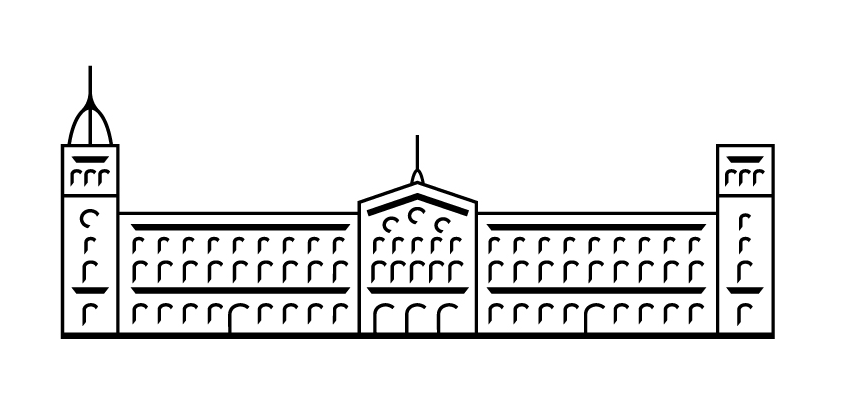
\includegraphics[width=13mm]{./ub}} \end{picture} } 
\fancyhead[LO]{ \begin{picture}(0,0) \put(0,-3){
\includegraphics[width=8mm]{./upc}} \end{picture} \quad \quad \begin{picture}(0,0) \put(0,-3){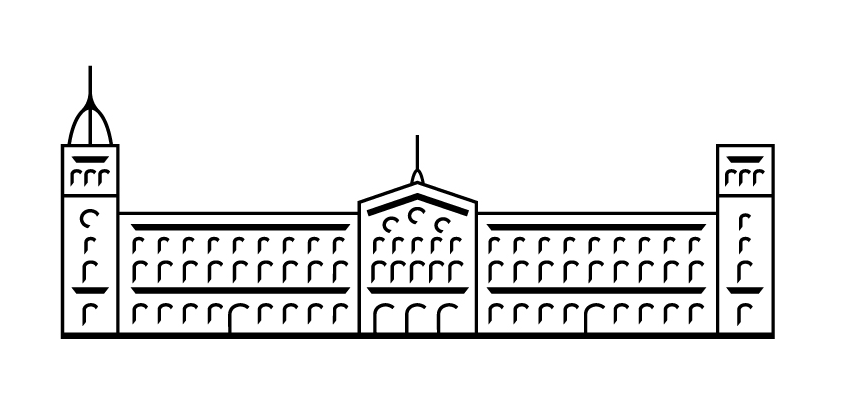
\includegraphics[width=13mm]{./ub}} \end{picture} \quad \quad \quad \begin{picture}(0,0) \put(0,-3){
\includegraphics[width=9mm]{./urv}} \end{picture} \quad \quad  \quad\small{MAI} }
%\fancyhead[LO]{\begin{picture}(0,0) \put(0,-3){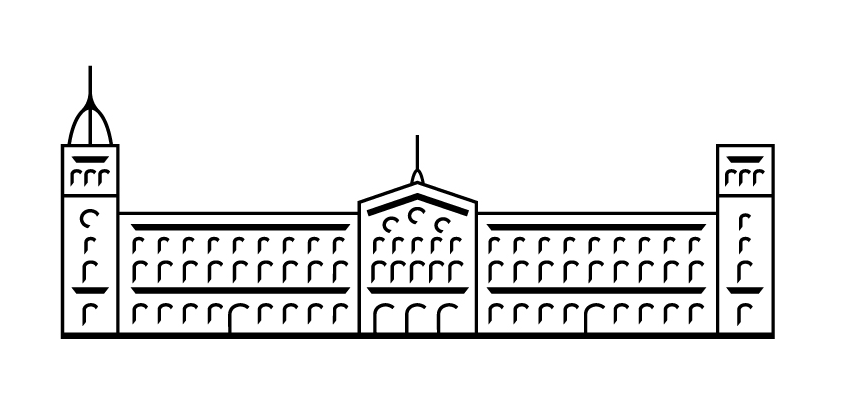
\includegraphics[width=13mm]{./ub}} \end{picture} \quad \quad \quad \small{Universitat de Barcelona} }
%\fancyhead[CE,CO]{\begin{picture}(0,0) \put(-17.01,-4.2){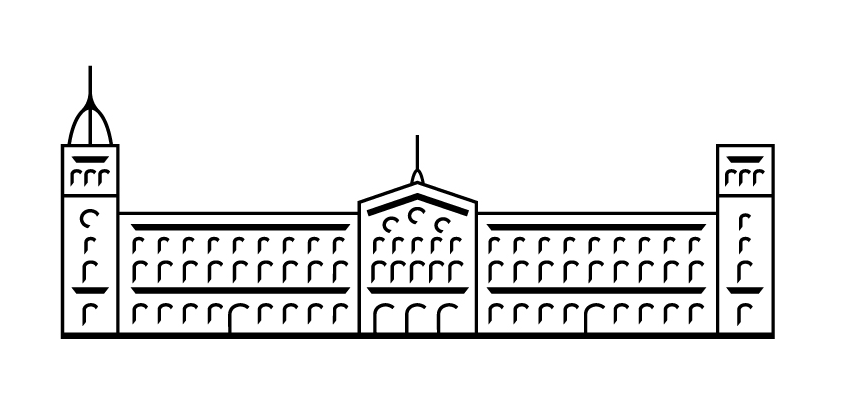
\includegraphics[width=12mm]{./ub}} \end{picture}} %foto de la ub en medio del encabezado
\fancyfoot[CO,CE]{}
\fancyfoot[RO,LE]{\thepage}

\fancypagestyle{plain}{%
\fancyhf{} % clear all header and footer fields
\fancyfoot[RO,LE]{\thepage} % except the center
\renewcommand{\headrulewidth}{0pt}
\renewcommand{\footrulewidth}{0pt}}

\setcounter{secnumdepth}{3}
\setcounter{tocdepth}{3} 
\usepackage{xcolor}
\usepackage[colorlinks = true,
            linkcolor = blue,
            urlcolor  = blue,
            citecolor = blue,
            anchorcolor = blue]{hyperref}

%--------------------------------------------------

\begin{document}


\thispagestyle{empty}

\begin{titlepage}

\begin{center}
	\vspace*{1cm}
	\rule{16cm}{0.2mm}\\
	\vspace*{0.4cm}
	\Huge{\textbf{Log-Distributional Approach for Learning Covariate Shift Ratios}}
	\rule{16cm}{0.2mm}\\
	\vspace{1cm}

	\Large{\textbf{Author: Guillermo Bernárdez Gil}}
\end{center}

\vspace{0.1cm}
\large{
\textbf{1$^{st}$ Advisor: Sergio Escalera}\\
\indent Departament de Matemàtiques i Informàtica \\ 
\indent Universitat de Barcelona

\vspace{8mm}
\textbf{2$^{nd}$ Advisor: Carles Gelada}\\
\indent Google Brain, Montreal \\
}
\vfill

\begin{center}
	\LARGE{A thesis presented for the degree of\\
	Master in Artificial Intelligence} \\
	\vspace{1cm}
	
\includegraphics[width=0.4\textwidth]{logo_upc.jpeg}
	
\includegraphics[width=0.4\textwidth]{logo_urv}
	\\ 
	
\includegraphics[width=4cm]{logo_ub}
	\\
	\large{Facultat d'Informàtica de Barcelona (FIB)} \\
	\large{Escola Tècnica Superior d'Enginyeria (URV)} \\
	\large{Facultat de Matemàtiques i Informàtica (UB)} \\
	\vspace{1cm}
	\Large{\today}
\end{center}

\end{titlepage}


\newpage
\pagenumbering{roman} 

\newpage 


\section*{Aknowledgements}

\newpage


\section*{Abstract}

Temporal Difference Learning algorithms classically learn value functions (sum of discounted rewards) by solving for the fixed point that relates the value of one state with the expected value of the following states. Other TD learning algorithms have been used to learn \textit{multiplicative value functions}, which also have a fixed point solution. An example of such a function is the ratio between stationary distributions of two policies. It has been shown that learning of these multiplicative value functions suffers from higher variance and looser convergence guarantees. One potential approach to solving this issues would be to learn in log space, turning the multiplicative value function into an additive one. Unfortunately, it is easy to show with Jensen's inequality that the exponential of the log fixed point does not correspond to the multiplicative fixed point.

Distributional RL has been used to learn the return distribution (return is the sum of future discounted rewards). Although it has been shown that it mainly plays an auxiliary task role for representation learning, we propose that distributional fixed points could play a much more fundamental role to learning non additive value functions. In the case of multiplicative value distributions, learning the additive fixed point in log space and exponentiating leads to the correct solution.

In particular, we will study this approach in the case of the learning process of the Covariate Shift Ratio, which defines a multiplicative value function.





\newpage

%\pagenumbering{roman} 
\tableofcontents

\newpage


\pagestyle{fancy}
\renewcommand{\sectionmark}[1]{\markboth{\thesection.\quad #1}{}}
\renewcommand{\subsectionmark}[1]{\markright{\thesubsection.\quad #1}}

\pagenumbering{arabic} 
\setcounter{page}{1}

\thispagestyle{plain}
\section{Introduction}

- Reinforcement Learning

- Distributional Reinforcement Learning

- Off-Policy Learning

- Covariate Shift Ratio


%\subsection*{Project}


\subsection*{Motivation and Goals}

- Relevance of logarithmic Distributional RL

- Dessign of Distributional Covariate Shift Ratio

- Evaluation of the logarithmich approach within the Distributional CSR setting


\subsection*{Structure of the Report}




\newpage


\thispagestyle{plain}
\section{Distributional Reinforcement Learning}




\subsection{Reinforcement Learning Setting}

Let's begin by characterizing our RL framework.

We consider an agent interacting with an environment in the standard setting\cite{rlformulation}: at each step $t$, the agent selects an action $a_t$ based on its current state $s_t$, to which the environment responds with a reward $r_t$ and then moves to the next state $s_{t+1}$. We model this interaction as a time-homogeneous Markov Decision Process $(\Sspace, \A, r, P, \gamma)$, where
\begin{itemize}
    \item $\Sspace$ and $\A$ are the state and action spaces, respectively, we assume that both are finite, with $n:=|\Sspace|$;
    \item $P$ is the transition kernel, $s_{t+1} \sim P(\cdot | s_t,a_t)$; the Markov assumption states that \\ $P(s_{t+1} | s_t, a_t, s_{t-1}, a_{t-1}, ...) = P(s_{t+1} | s_t, a_t)$;
    \item $r(s,a)$ represents the immediate reward given by the environment after taking action $a$ being in state $s$. These rewards are considered to be sampled from the reward function $R(s,a)$, i.e. $r_t \sim R(s_t,a_t)$;
    \item $\gamma$ is the discount factor
\end{itemize}

A policy $\pi$ maps each state to a probability distribution over the action space, $a_t \sim \pi(\cdot | s_t)$. In addition, we combine the policy $\pi$ and transition function $P$ into a state-to-state transition function $P_\pi \in \R^{n \times n}$ , whose entries are
\begin{equation} \label{transitionFunction}
    P_{\pi} (s'|s) := Prob_\pi (s_{t+1}=s' | s_t = s) = \sum_{a\in\A} \pi(a|s)P(s'|s,a)
\end{equation}
In particular, powers of $P_\pi$ represent the transition function across different time-steps.

Given $\pi$, the action value function is defined as the expected sum of discounted rewards from a state-action pair by following the policy:
\begin{equation} \label{AV}
Q^\pi (s,a) = \mathbb{E}_\pi \left[ \sum_{t=0}^\infty \gamma^t r(s_t,a_t) \bigg| s_0=s, a_0=a \right] 
\end{equation}
The Bellman's equation can be obtained from this expression:
\begin{equation} \label{BE}
\begin{split}
    Q^\pi (s,a) &= \mathbb{E} \left[ r(s,a) \right] + \gamma \E_\pi \left[ \sum_{t=0}^\infty \gamma^t r(s_{t+1},a_{t+1}) \bigg| s_0=s, a_0=a \right] \\
    &= \mathbb{E} \left[ r(s,a) \right] + \gamma \sum_{s'} P(s'|s,a) \left( \E_\pi \left[ \sum_{t=0}^\infty \gamma^t r(s_{t+1},a_{t+1}) \bigg| s_1=s' \right] \right) \\
    &= \mathbb{E} \left[ r(s,a) \right] + \\
    & \quad \gamma \sum_{s'} P(s'|s,a) \sum_{a'} \pi(a'|s')\left( \E_\pi \left[ \sum_{t=0}^\infty \gamma^t r(s_{t+1},a_{t+1}) \bigg| s_1=s', a_1=a' \right] \right)\\
    %&= \mathbb{E} \left[ r(s,a) \right] + \gamma \sum_{s'} P(s'|s,a) \sum_{a'} \pi(a'|s') Q(s',a') \\
    &= \mathbb{E} \left[ r(s,a) \right] + \gamma \E_{s'\sim P(\cdot | s,a), a' \sim \pi(\cdot | s')} \bigg[Q(s',a') \bigg] \\
\end{split}
\end{equation}


Analogously for the state value function (considering $r_\pi(s) := \mathbb{E}_{a\sim\pi(\cdot | s)} \left[ r(s,a) \right]$):
\begin{equation} \label{SV}
\begin{split}
    V^\pi (s) &= \mathbb{E}_\pi \left[ \sum_{t=0}^\infty \gamma^t r(s_t,a_t) \bigg| s_0=s\right] \\
    &= r_\pi(s) + \gamma \sum_a \pi(a | s) \sum_{s'} P(s'|s,a) \left( \E_\pi \left[ \sum_{t=0}^\infty \gamma^t r(s_{t+1},a_{t+1}) \bigg| s_1=s' \right] \right) \\
    &= r_\pi(s) + \gamma \E_{s'\sim P_{\pi}(\cdot | s)} \bigg[V^\pi(s') \bigg]
\end{split}
\end{equation}


\subsubsection*{Policy Evaluation vs. Control Setting}

Typically, we can distinguish two different settings among -and within- RL algorithms. On the one hand, we may be interested in computing the value function, assuming the current policy $\pi$ is fixed, so as to evaluate that policy (\textit{policy evaluation}). On the other hand, we might want to actually improve the current policy (\textit{control setting}). Both settings have been extensively analyzed (e.g. \cite{TD}) and have associated their corresponding Bellman operators.


In the context of \textit{policy evaluation}, considering state-action value functions $Q^\pi$ as vectors in $\R^{\Sspace \times \A}$, the \textit{Bellman operator} $\T^{\pi} : \R^{\Sspace \times \A} \rightarrow \R^{\Sspace \times \A}$ is defined as
\begin{equation} \label{BellmanOp}
	{\T}^\pi Q(s,a) :=  \mathbb{E} \left[ r(s,a) \right] + \gamma \E_{s'\sim P(\cdot | s,a), a' \sim \pi(\cdot | s')} \bigg[Q(s',a') \bigg]
\end{equation}
Such operator is useful to describe the expected behaviour of popular learning algorithms (e.g. Q-learning) and satisfies some interesting and desirable properties\cite{rlformulation}:
\begin{itemize}
	\item It is a contraction mapping (see Appendix \ref{contractionTheory})
	\item The process $Q_t = \T^\pi Q_{t-1}$, for some initial value $Q_0$, converges exponentially to $Q^\pi$ as $t \rightarrow \infty$.
\end{itemize}


Regarding the \textit{control setting}, where the goal is to improve the current policy $\pi$, a \textit{Bellman optimality operator} $\T^* : \R^{\Sspace \times \A} \rightarrow \R^{\Sspace \times \A}$ is defined as follows:
\begin{equation} \label{BellmanOptimalityOp}
	{\T}^* Q(s,a) :=  \mathbb{E} \left[ r(s,a) \right] + \gamma \E_{s'\sim P(\cdot | s,a)} \bigg[ \max_{a' \in \A}  Q(s',a') \bigg]
\end{equation}
As it was shown in \cite{rlformulation}, $\T^*$ is also a contraction mapping, and the expectation of $\{ Q_t \}$, $Q_t = \T^* Q_{t-1}$, converges exponentially to a fixed point (in this case, the optimal value function $Q^*$).

\subsection{Towards a Distributional Reinforcement Learning}

Now that we have introduced the standard expected-based RL setting, we go a step further and present its distributional counterpart, which has become the focus of many RL research from the publication of \cite{DRL}.

The first key of that work is to redefine the RL framework from a distributional perspective; we are not dealing with expected values anymore, but with proper distributions. Bearing that in mind, they define the following distributional Bellman equation:
\begin{equation} \label{distBE}
    Z^{\pi}(s,a) \stackrel{D}{=} R(s,a) + \gamma Z^{\pi}(S',A'),
\end{equation}
where
\begin{itemize}
    \item $Z^\pi: \Sspace \times \A \rightarrow \Z$ is the \textit{value distribution}, a mapping from state-action pairs to distributions over returns by following policy $\pi$. Its expectation is the value $Q^\pi$
    	\begin{equation} \label{QexpZ}
        		Q^\pi(s,a) := \mathbb{E} [Z^\pi(s,a)]
    	\end{equation}
    	We will also call it the \textit{return distribution}.
    \item $(S',A') \in \Sspace \times \A$ is the next state-action random variable: $S'\sim P(\cdot | s,a)$, $A' \sim \pi(\cdot | S')$
    \item $R(s,a) \in \Z$ is the random reward, or equivalently the reward function. Note that now we are dealing with it as an explicit random variable.
    \item $Z^\pi(S',A') \in \Z$ is the random return over the random next state-action following $\pi$. This notation implies that all possible next state-action pairs need to be considered as to generate this return distribution. Thus, $Z^\pi(S',A')$ may be seen as a mixture distribution of the distributions $Z^\pi(s',a')$ where $s'$ and $a'$ are sampled from $(S',A')$:
    \begin{equation}
        f_{Z^\pi(S',A')} (z) = \sum_{s'} P(s' | s,a) \sum_{a'} \pi(a'|s') f_{Z^\pi(s',a')}(z)
    \end{equation}
    The expected value, using \ref{QexpZ}, can be then expressed as:
    \begin{equation} \label{expNextRandomReturn}
    \begin{split}
        \E[Z^\pi(S',A')] &=  \int_{-\infty}^{\infty} z \sum_{s'} P(s' | s,a) \sum_{a'} \pi(a'|s') f_{Z^\pi(s',a')}(z) dz \\
        &=  \sum_{s'} P(s' | s,a) \sum_{a'} \pi(a'|s') \int_{-\infty}^{\infty} z f_{Z^\pi(s',a')}(z) dz \\
        &=  \sum_{s'} P(s' | s,a) \sum_{a'} \pi(a'|s') \E[Z^\pi(s',a')] \\
        &= \E_{s'\sim P(\cdot | s,a), a' \sim \pi(\cdot | s')} \bigg[Q^\pi(s',a') \bigg] 
    \end{split}
    \end{equation}
\end{itemize}

\begin{remark}
A distributional equation $U \stackrel{D}{:=} V$ indicates that the random variable $U$ is distributed according to the same law as $V$.	
\end{remark}

Note that we can easily recover the classical Bellman's equation \ref{BE} for the action value Q by using \ref{QexpZ} and \ref{expNextRandomReturn} when taking the expected value over its distributional version \ref{distBE}:
\begin{equation}
\begin{split}
    Q^\pi(s,a) &= \mathbb{E} [Z^\pi(s,a)] \\
    &= \E[R(s,a)] + \gamma \E[Z^\pi(S',A')] \\
    &= \mathbb{E} [r(s,a)] + \gamma \E_{s'\sim P(\cdot | s,a), a' \sim \pi(\cdot | s')} \bigg[Q^\pi(s',a') \bigg] 
\end{split}
\end{equation}

Finally, let's try to find out what actually the random return $Z$ represents by expanding its density function: 
\begin{equation} \label{meaningZ}
\begin{split}
    f_{Z^\pi(s,a)}(z) &= f_{R(s,a) + \gamma Z^\pi(S',A')}(z)  \\
    &=  \sum_{s'} P(s' | s,a) \sum_{a'} \pi(a'|s') f_{R(s,a) + \gamma Z^\pi(s',a')}(z) \\
    &= \sum_{s'} P(s' | s,a) \sum_{a'} \pi(a'|s') f_{R(s,a) + \gamma (R(s',a') + \gamma Z^\pi(S'',A''))}(z) \\
    &= \sum_{s'} P(s' | s,a) \sum_{a'} \pi(a'|s') \sum_{s''} P(s'' | s',a') \sum_{a''} \pi(a''|s'') \\
    & \quad \quad f_{R(s,a) + \gamma R(s',a') + \gamma^2 Z^\pi(s'',a'')} (z) \\
    &= \sum_{s_{1}} P(s_{1} | s_{0},a_{0}) \sum_{a_{1}} \pi(a_{1}|s_{1})  \cdots \sum_{s_{t}} P(s_{t} | s_{t-1},a_{t-1}) \sum_{a_{t}} \pi(a_{t}|s_{t}) \\
    & \quad \quad f_{\sum_{i=0}^{t} \gamma^t R(s_{t},a_{t})} (z)
\end{split}
\end{equation}
where we have repeatedly used property \ref{mixtureProperty2} of mixture distributions. In addition, note that assuming independence between the random reward $R$ of a certain state-action pair and the return distribution $Z^\pi$ of the possible next state-action (which is NOT TRUE in general), we can rewrite it in terms of convolutions as
\begin{equation}
\begin{split}
    f_{Z^\pi(s,a)}(z) &= \sum_{s_{1}} P(s_{1} | s_{0},a_{0}) \sum_{a_{1}} \pi(a_{1}|s_{1})  \cdots \sum_{s_{t}} P(s_{t} | s_{t-1},a_{t-1}) \sum_{a_{t}} \pi(a_{t}|s_{t}) \\
    & \quad \quad  \left( f_{R(s_0,a_0)} * f_{\gamma R(s_1,a_1)} *  \cdots * f_{\gamma^t R(s_{t},a_{t})} \right) (z)
\end{split}
\end{equation}

According to \ref{meaningZ}, $Z^{\pi}(s,a)$ can be interpreted as a convex combination of the sum of discounted reward distributions of all possible agent trajectories starting at the state-action $(a,s)$ and following policy $\pi$ from then on, each weight corresponding to the probability of that precise trajectory. It is important to note that $Z^\pi$ encodes the intrinsic randomness of the agent's interactions with its environment; we should avoid considering it as a measure of uncertainty about the environment itself.

Moving to the \textit{policy evaluation} setting, now we are interested in studying the behaviour of a distributional version of the policy evaluation operator $\T^\pi$. First we define the transition operator $P^\pi : \Z \rightarrow \Z$ 
\begin{equation} \label{distTransitionOp}
	P^\pi Z(s,a) \stackrel{D}{:=} Z(S',A')
\end{equation}
Given this, the \textit{distributional Bellman operator} $\T : \Z \rightarrow \Z$ is defined as
\begin{equation} \label{distBellmanOp}
	{\T}^\pi Z(s,a) \stackrel{D}{:=} R(s,a) + \gamma P^{\pi} Z(s,a)
\end{equation}
We emphasize that three sources of randomness are involved in the compound distribution ${\T}^\pi Z$, i.e.
\begin{enumerate}
	\item Randomness in the reward $R$,
	\item Randomness in the transition $P^\pi$, and
	\item Randomness in the next state-value distribution $Z(S', A')$,
\end{enumerate} 
which together make this distributional Bellman operator fundamentally different to the expected value-cased one (Equation \ref{BellmanOp}). Authors in \cite{DRL} demonstrate, under the assumption that these three random quantities are independent, that ${\T}^\pi$ is a contraction mapping whose unique fixed point is the value distribution $Z^\pi$.


However, more difficulties arise in the \textit{control setting} when dealing with this distributional perspective; as stated in \cite{DRL}, while every optimal policy attain the same value $Q^*$ in the expected-valued case, there might be many optimal value distribiutions. Considering the set $\Pi^*$ of optimal policies, an optimal value distribution is defined as the value distribution of an optimal policy. Hence, the set of optimal value distributions is $\Z^* := \{ Z^{\pi^*} : \pi^* \in \Pi^* \}$.

Note that an optimal value distribution must match the full distribution of returns under some optimal policy, so that not all value distributions with expectation $Q^*$ are optimal. A \textit{distributional Bellman optimality operator} $\T$ is defined as well, but it doesn't behave as well as the policy evaluation operators: it is not a contraction in any usual metric between distributions, and its convergence to the set of optimal value distributions is weak.



\subsection{Approximation Framework in the Distributional Setting} \label{aproxFramework}

%Let $\Ppi (s,a)$ be the distribution of the random variable $Z^\pi (s,a)$. The process of learning $\Ppi$ 
We should we aware that the full computation of the distributional Bellman operators on return distribution functions is generally either impossible (as we typically do not have access to the MDP dynamics, but to merely sample transitions) or infeasible (since the value distribution cannot be stored exactly in the general case).

This lead us to the design of several key approximations which are required to implement practical and scalable distributional RL algorithms\cite{analysisC51}:

\subsubsection*{Distribution Parametrisation}
Due to the fact that the full space of probability distributions, $\mathscr{P}(\R)$, cannot be algorithmically encoded with a finite number of parameters, we need to approximate the distribution throughout a parametric family $\mathcal{P} \in \mathscr{P}(\R)$.

\subsubsection*{Stochastic Bellman Operators}
In order to evaluate the distributional Bellman operator $\T^\pi$, all possible next state-action-reward combinations should be taken into account. As in the expected valued case, the usual way of overcoming this practical limitation is by learning through transition samples $(s,a,r,s',a')$ of the MDP. Hence, we can define a \textit{stochastic distributional Bellman operator} $\widehat{\T}^\pi$ adapted to the randomness of these transitions, which defines a random measure whose behaviour is equal in expectation to the true Bellman operator $\T^\pi$. %In our theoretical development, for the sake of simplicity, we will consider the simpler setting where stochastic operators are not needed.

\subsubsection*{Projection of Bellman Target Distribution}
Another problem usually arises after computing the stochastic operator $\widehat{\T}^\pi$ over a value distribution $Z(s,a)$: the new distribution may no longer lie in the selected parametric family $\mathcal{P}$. If this is the case, we further need to apply a \textit{projection operator} $\Pi : \mathscr{P}(\R) \rightarrow \mathcal{P}$ so as to map $\widehat{\T}^\pi Z(s,a)$ into the proper parametric family.

\subsubsection*{Gradient Updates}
 Finally, having computed a stochastic approximation $\widehat{Z}_k (s_k,a_k) = \Pi \widehat{\T}^\pi Z_k(s_k,a_k)$ to the full target distribution, we still have to define how to compute the next iterate $Z_{k+1}$. For that, the use of gradient updates seems to be appropiate\cite{rlformulation}, as it helps dissipate some noise introduced in the target by the stochastic approximation. A key aspect here, however, is the not-straightforward correspondence between the considered loss and the previously selected projection; convergence and good behaviour of the resulting algorithm have only be proven when both of them rely on the same norm-induced geometry\cite{analysisC51,rlformulation}

\subsection{Categorical Distributional Reinforcement Learning}

Although the distributional perspective is almost as old as Bellman's equations\cite{firstDistributional}, it was not until the recent introduction of the Categorical Distributional Reinforcement\cite{DRL} (CDRL) that it has become a central role within reinforcement learning. Their algorithm, called C51, was able to obtain state-of-the-art results in the Arcade Learning Environment\cite{ALE} (ALE), outperforming the top expected-valued solutions by then.

The name 'categorical' comes from the distribution parametrisation that is used, which consists in the parametric family of categorical distributions over some fixed set of equally-spaced supports $z_1 < \cdots < z_K$:
\begin{equation}
	\mathcal{P} = \left\{ \sum_{i=1}^{K} p_i \delta_{z_i} \Big| p_1, \dots , p_K \geq 0, \sum_{k=1}^{K} p_k = 1 \right\}
\end{equation}
Apart from that, the algorithm can be fully characterized by the rest of approximations implemented within the distributional RL framework described in the previous subsection:
\begin{itemize}
	\item So as to learn from sampling transitions, we move to the \textit{stochastic distributional Bellman operator} $\widehat{\T}^\pi$ and the \textit{stochastic distributional Bellman optimality operator} $\widehat{\T}^*$. Given a sampled transition $(s_t,a_t,r,s_{t+1},a_{t+1})$, these stochastic operators basically transform the supports of the distributions by an affine shift map $f_{r,\gamma} : \R \rightarrow \R$, defined by $f_{r,\gamma}(z) = r + \gamma z$; in our notation, 
		$$\widehat{\T} Z_t(s_t,a_t) = (f_{r,\gamma})_\# Z_t(s_{t+1},a_{t+1})$$
		with $a_{t+1}$ either being selected by sampling the policy $\pi(\cdot | s_{t+1})$  (categorical policy evaluation, i.e. $\widehat{\T}=\widehat{\T}^\pi$), or being the action with the highest estimated expected returns (categorical Q-learning, $\widehat{\T}=\widehat{\T}^*$).
		
	\item CDRL applies the heuristic projection operator $\Pi_C$ after computing the stochastic Bellman operators in order to recover a distribution within the selected parametric family $P$. This projection is defined for single Dirac measures as
	\begin{equation} \label{heuristicProjectionOp}
		\Pi_C (\delta_y) = \left\{
		\begin{array}{ll}
			\delta_{z_1} & y\leq z_1 \\
			\\ \frac{z_{i+1} -y}{z_{i+1}-z_i} \delta_{z_i} + \frac{y-z_i}{z_{i+1}-z_i} \delta_{z_{i+1}} & z_i < y < z_{i+1} \\
			\\ \delta_{z_K} & y>z_K
		\end{array}
		\right.
	\end{equation}
	and can be easily extended to finite mixtures of Dirac measures: 
	$$ \Pi_C \left( \sum_{i=1}^{N} p_i \delta_{y_i} \right) = \sum_{i=1}^{N} p_i \Pi_C ( \delta_{y_i} )	$$
	This projection step provides us with the target $\widehat{Z}_t (s_t,a_t) = \Pi_{C} \widehat{\T} Z_t(s_t,a_t)$. 
	
	%In addition, we will also denote by $\Pi_C$ the operator $\mathscr{P}(\R)^{\Sspace \times \A} \rightarrow \mathcal{P}^{\Sspace \times \A}$ that applies this projection to each distribution in the return distribution function.
	
	\item Finally, the original C51 performs a single step of gradient descent on the Kullback-Leibler divergence (see Appendix \ref{metrics} for the definition of this metric) of the prediction $Z_t(s_t,a_t)$ from the target $\widehat{Z}_t (s_t,a_t)$:
	$$ \textnormal{KL} \left( \widehat{Z}_t (s_t,a_t) || Z_t (s_t,a_t) \right) $$
	with respect to the parameters of $Z_t (s_t,a_t)$; this gradient is used to generate the new estimate $Z_{t+1}(s_t,a_t) = \sum_{k=1}^{K} p_{t+1,k}(s_t,a_t) \delta_{z_k}$.
	
\end{itemize}

Pseudo-Algorithm \ref{CDRL} (provided by \cite{analysisC51}) synthesises the steps performed by CDRL.

\setlength{\algomargin}{1.5em}
\SetAlCapHSkip{0em}
\begin{algorithm}[H]
\caption{Categorical Distributional Reinforcement Learning} \label{CDRL}
\DontPrintSemicolon
\SetKwComment{CustomComment}{\#}{}
\SetKwInput{KwIn}{\hspace{-1.5em} Input}
\SetKwInput{KwOut}{\hspace{-1.5em} Output}
\SetKwInOut{Require}{\hspace{-1.5em} Require}
\Require{$Z_t(s,a) = \sum_{k=1}^K p_{t,k}(s,a) \delta_{z_k}$ for each $(s,a)$}
\KwIn{A sample transition $(s_{t},a_{t}, r_t, s_{t+1})$}
	\CustomComment{Compute distributional Bellman target}
    \uIf{\textnormal{Categorical Policy Evaluation}}{
    	$a^* \sim \pi(\cdot | s_{t+1})$ \;}
    \ElseIf{\textnormal{Categorical Q-learning}}{
    	$a^* \leftarrow \textnormal{arg max}_a Q(s_{t+1},a) $\;}
    $\widehat{Z}_{*}(s_t,a_t) \leftarrow (f_{r_t,\gamma})_{\#} Z_t(s_{t+1},a^*)$\;
    \CustomComment{Project target onto support}
    $\widehat{Z}_{t}(s_t,a_t) \leftarrow \Pi_C \widehat{Z}_{*}(s_t,a_t)$\;
    \CustomComment{Compute KL loss}
    \textnormal{Find gradient }$ \textnormal{KL} \left( \widehat{Z}_t (s_t,a_t) || Z_t (s_t,a_t) \right) $\; 
    \textnormal{Generate new estimate }$Z_{t+1}(s_t,a_t) = \sum_{k=1}^{K} p_{t+1,k}(s_t,a_t) \delta_{z_k}$ \;
\KwOut{Estimate $Z_{t+1}(s,a)$ for each $(s,a)$}

\end{algorithm}


Despite the good results obtained by C51, all attempts to prove its convergence have failed so far. One of its most controversial steps, at least from a theoretical point of view, is the use of the KL divergence while applying the heuristic projection $\Pi_{C}$; as shown in \cite{analysisC51}, using the Cramér distance instead allows a useful geometrical reinterpretation of $\Pi_{C}$ that lead us to the desired convergence results.

In fact, we recall that authors in \cite{DRL} demonstrates, in the context of policy evaluation setting, that applying the Bellman operator $T^{\pi}$ repeatedly to an initial return distribution function $Z_0$ guarantees convergence to the true set of return distributions $Z^\pi$ in the supremum-Wasserstein metric. They did so by showing that
\begin{lemma} \label{contractiondp}
	$\T^\pi : \Z \rightarrow \Z$ is a $\gamma$-contraction in $\bar{d}_p$
\end{lemma}

However, after the introduction of the parametrization $\mathcal{P}$ and the projection operator $\Pi_C$, it is important to note that the operator to be analyzed is not the Bellman operator $\T^\pi$ itself anymore, but its composition with the projection operator, i.e. $\Pi_C \T^\pi$. As stated in \cite{analysisC51}, this can make contractivity break under all Wasserstein distances but $\bar{d}_1$ :
\begin{lemma} \label{nocontractiondp}
	$\Pi_C \T^\pi : \Z \rightarrow \Z$ is in general not a contraction in $\bar{d}_p$, for $p>1$
\end{lemma}

In contrast to that, Cramér distance seems to induce a useful geometric structure on the space of probability measures, allowing us to establish contractivity of the combined operator $\Pi_C \T^\pi$ in a much more natural way. We dedicate the following two sections to analyze CDRL algorithms together with Cramér-based metrics in the case of both Tabular Representations and Linear Function Approximations, respectively, which are the theoretical frameworks where stable behaviour and convergence properties are proven so far.


\subsubsection{Tabular Representation} \label{CDRLtabular}

Our first approach to study Cramér-based CDRL algorithms will be to consider the simplest reinforcement learning framework, where we are able to store an approximate parametrization distribution for each state-action pair: the so-called tabular case.

Again, we will consider the parametric family $\mathcal{P}$ of categorical distributions over some fixed support $\{z_1, \dots , z_K\}$, as well as the heuristic projection operator $\Pi_C$ defined in Equation \ref{heuristicProjectionOp} for mapping the backup distribution function $\T^\pi Z$ into $\mathcal{P}$. However, for the sake of simplicity and understandability, we will assume that no stochastic approximation is required. 

First of all, we present the result of \cite{analysisC51} that motivates the use of Cramér distance, which shows an interesting connection between this distance and the projection operator $\Pi_C$:
\begin{prop} \label{CramerProj}
	The Cramér metric $\ell_2$ endows a particular subset of $\mathscr{P}(\R)$ with a notion of orthogonal projection, and the orthogonal projection onto the subset $\mathcal{P}$ is exactly the heuristic projection $\Pi_C$. Consequently, $\Pi_C$ is a non-expansion with respect to $\ell_2$.
\end{prop}

The previous proposition directly lead us to the contractivity of the operator $\Pi_C \T^\pi$, which in turn ensures its convergence in the absence of stochastic approximation:
\begin{prop} \label{CramerBellmanContraction}
	The operator $\Pi_C \T^\pi$ is a $\sqrt{\gamma}$-contraction in $\bar{\ell}_2$. Further, there is a unique distribution function $Z_C \in \mathcal{P}^{\Sspace \times \A}$ to which the process $Z_{k+1} := \Pi_c \T^\pi Z_k$, given any initial distribution function $Z_0 \in \mathscr{P}(\R)^{\Sspace \times \A}$, converges in $\bar{\ell}_2$ as $k \rightarrow \infty$.
\end{prop}

Authors in \cite{analysisC51} also address the natural question of how the limiting distribution function $Z_C$ can differ from the true return distribution $Z^\pi$:
\begin{prop} \label{errorTabular}
	Let $Z_C$ be the limiting return distribution of Proposition \ref{CramerBellmanContraction}. If for all state-action pairs their corresponding true return distribution $Z^\pi$ is supported on $[z_1,z_K]$, then 
	$$\bar{\ell}_2(Z_C, Z^\pi) \leq \frac{1}{1-\gamma} \max_{1\leq i \leq K} (z_{i+1}-z_i). $$
\end{prop}
Note that the true return distribution is gradually recovered as the fineness of the support increases. Hence, this result can be viewed as a way of quantifying the cost of using the parametrization $\mathcal{P}$ instead of fully non-parametric probability distributions. Finally, we also highlight the assumption that the support of the true return distributions lie on the selected support, since we don't always have access to the scale of rewards in every RL problem; for these circumstances, an analogous result can be found in Proposition 4 of \cite{analysisC51}.

\begin{comment}
\setlength{\algomargin}{1.5em}
\SetAlCapHSkip{0em}
\begin{algorithm}[H]
\caption{CDRL with Tabular Representation} \label{tabularCDRL}
\DontPrintSemicolon
\SetKwComment{CustomComment}{\#}{}
\SetKwInput{KwIn}{\hspace{-1.5em} Input}
\SetKwInput{KwOut}{\hspace{-1.5em} Output}
\SetKwInOut{Require}{\hspace{-1.5em} Require}
\Require{$Z_t(s,a)$ for each $(s,a)$}
\KwIn{A state-action pair $(s_{t},a_{t})$}
	\CustomComment{Compute distributional Bellman target}
    \uIf{\textnormal{Categorical Policy Evaluation}}{
    	$\widehat{Z}(s_t,a_t) \leftarrow \T^\pi Z_t(s_{t},a_{t})$\;}
    \ElseIf{\textnormal{Categorical Q-learning}}{
    	$\widehat{Z}(s_t,a_t) \leftarrow \T^* Z_t(s_{t},a_{t})$\;}
    \CustomComment{Project target onto support}
    $\widehat{Z}_{t}(s_t,a_t) \leftarrow \Pi_C \widehat{Z}(s_t,a_t)$\;
    \CustomComment{Update estimate}
    $Z_{t+1}(s_t,a_t) \leftarrow \widehat{Z}_{t}(s_t,a_t)$ \;
\KwOut{Estimate $Z_{t+1}(s,a)$ for each $(s,a)$}
\end{algorithm}
\end{comment}


\subsubsection{Linear Function Approximation} \label{CDRLlinear}

In this second and last theoretical approach, we go a step beyond the tabular case by considering a framework where we make use of function approximators to compute the parametrized return distributions of each state-action pair, assuming a more realistic situation in which the state space is too large to store individual distributions.

We will restrict our analysis to the context of linear function approximation, whose convergence is already proven in \cite{DRLlinear}. To the best of our knowledge, no Distributional RL algorithm with a non-linear function approximator has been proven to converge so far, despite the many efforts in studying C51.

Regarding the rest of approximations and assumptions of the CDRL algorithms considered in this study, they are exactly the same as in the previous Section \ref{CDRLtabular}: we contemplate the parametric family $\mathcal{P}$ with fixed support $\{z_1, \dots, z_K\}$, the Cramér-based projection $\Pi_C$, and reject any stochastic approximation.

In our linear model, we now redefine the approximated return distributions $Z$ as mappings from states $s\in \Sspace$ to vectors defined by a linear combination of features:
\begin{equation}
	Z_{\Theta}(s) := \Theta^\top \phi(s)
\end{equation}
where $\phi(s)\in \R^m$ is the feature vector at state $s$ and $\Theta \in \R^{n\times K}$ represents the weight matrix. Therefore, we are assuming that the vector $Z_{\Theta}(s) \in \R^{K}$ is an estimation of a distribution over the support $\{z_1,\dots,z_K\}$, although it might have negative components and it is not necessarily normalized. 

\begin{notation}
	In vector notation, we will write $Z_{\Theta} = \Phi \Theta \in \R^{n\times K}$, where $\Phi \in \R^{n \times m}$ is the feature matrix, simply formed by all feature vectors.
\end{notation}


Before continuing, let's carefully review the three different spaces of distributions-like objects that we face in CDRL with linear function approximation:
\begin{itemize}
	\item On the one hand, we have the probability space where true return distributions lie; without any prior knowledge, we should simply consider the full space of distributions $Z^\pi \in \mathscr{P}(\R)$. Assuming that we know \textit{a priori} the scale of the rewards, we can reduce it to the space of distributions with support in a certain interval; in our case, it could be $Z^\pi \in \mathscr{P}([z_1,z_K])$.
	\item On the other hand, the selected parametric family $\mathcal{P}$ of categorical distributions over the support $\{z_1,\dots,z_K\}$; so far, we have expected our estimated return distributions $Z$ to belong to this space, $Z \in \mathcal{P}$.
	\item Finally, and in addition to the previous two, we now have a new vector space spanned by the features $\Phi \in \R^{n\times m}$, i.e. $\mathcal{L} := \{ \Phi\Theta : \Theta \in \R^{m\times K}\}$. This is, in fact, the crucial space in our development, as every approximated return distribution $\Z_{\Theta}$ lies in it. Ideally, if all $Z_\Theta$ were proper probability distributions over $\{z_1,\dots,z_K\}$, we would have $\mathcal{L} \subset \mathcal{P}$ (assuming some loss of expressiveness by our linear model).
\end{itemize}

%This can be seen in Pseudo-algorithm \ref{linearCDRL}, which defines the process of linear-based CDRL step by step. 
Let's review the process. First, our linear function model provides us with return distribution estimates 
$$Z_\Theta \in \mathcal{L}$$
 for each state $s \in \Sspace$. In order to get better approximations, CDRL algorithm applies the distributional Bellman operator, so we get
 $${\T}^\pi Z_{\Theta} \in \mathscr{P}([z_1,z_K]).$$
 Then we would need to apply a first projection operator $\Pi_1 : \mathscr{P}([z_1,z_K]) \rightarrow \mathcal{P}$ (like the Cramér projection $\Pi_C$) so as to recover a distribution within our selected parametric family, so
 $$\Pi_1 {\T}^\pi Z_{\Theta} \in \mathcal{P}.$$
 However, for the algorithm to compare distributions and improve its linear representations, now we need a further projection onto the space $\mathcal{L}$, which defines all the probability distributions that our linear model can actually express. Thus, the idea is that a second projection operator $\Pi_{2} : \mathcal{P} \rightarrow \mathcal{L}$ is required so that
 $$\Pi_2 \Pi_1 {\T}^\pi Z_{\Theta} \in \mathcal{L}.$$
As shown in \cite{DRLlinear}, the (re)definition of both projections plays again a very important role for proving the convergence of the process $Z_{\Theta_{k+1}} = \Pi_2 \Pi_1 {\T}^\pi Z_{\Theta_{k}}$. 

So far, we demonstrated in the tabular case that the combined operator $\Pi_C \T^\pi$ is a contraction mapping in the supremum-Cramér metric $\bar{\ell}_2$; our task now is to achieve a similar result for the combination $ \Pi_2 \Pi_1 {\T}^\pi$. For doing so, authors in \cite{DRLlinear} introduce a \textit{generalized Cramér distance} which is able to deal with our return distribution estimates (we recall they are not necessarily probability distributions).

We denote by $C\in \R^{K\times K}$ the lower-triangular matrix of ones, and by $e\in\R^K$ the vector of ones. Let $e_K= (1/\sqrt{K}) e^\top$ and $\Pi_{e_K^\top} = I_K - e_K e_K^\top$. For any two discrete value distributions $Z_1, Z_2$ over the fixed support $\{z_1,\dots,z_K\}$, the generalized Cramér distance is defined as
\begin{equation} \label{generalizedCramer}
	\ell_{\lambda}^2(Z_1,Z_2) = (Z_1 - Z_2)^\top \Pi_{e_K^\top} C C^\top \Pi_{e_K^\top} (Z_1 - Z_2) + \lambda ((Z_1 - Z_2)^\top e_K)^2 
\end{equation}
We will simplify the notation by denoting $C_\lambda = \Pi_{e_K^\top} C C^\top \Pi_{e_K^\top} + \lambda e_K e_K^\top $, so we can rewrite the distance definition as 
\begin{equation*}
	\ell_{\lambda}^2(Z_1,Z_2) = (Z_1 - Z_2)^\top C_\lambda (Z_1 - Z_2) = \| Z_1 - Z_2 \|_{C_\lambda}
\end{equation*}
\begin{comment}
It can be extended to the continuous case by
\begin{equation} \label{contGeneralizedCramer}
\begin{split}
	\ell_{\lambda}^2(Z_1,Z_2) = &\int_{x=z_1}^{z_K} \left( \int_{y=z_1}^{x} [ \Pi_{e^\perp} Z_1(y) - \Pi_{e^\perp} Z_2(y) ] dx \right)^2 dy \ + \\
	&\lambda \left( \int_{y=z_1}^{z_K} [Z_1(y) - Z_2(y)] dx \right)^2
\end{split}
\end{equation}
where for each return distribution $Z$
\begin{equation*}
	 \Pi_{e^\perp} Z(x) = Z(x) - \int_{y=z_1}^{z_K} Z(y) dy.
\end{equation*}
\end{comment}
Looking at Equation \ref{generalizedCramer}, the idea is that the first term on the right-hand side penalizes the difference in cumulative probabilities of both distributions, whereas the second term accounts for the difference in mass; we refer to \cite{DRLlinear} to get more details.

But, in addition to the Cramér distance generalization, authors in \cite{DRLlinear} also take into account the distribution $\xi$ according to which the states to be updated are sampled; %It can be whatever distribution, but in our case, given that we are following a policy $\pi$, we can consider it to be the stationary distribution $d_\pi$ (i.e. $d_\pi \in \Delta(\Sspace)$ such that $d_\pi = P_\pi d_\pi$; see a more detailed definition in Section \ref{COPTDsetting}).
they use it to define a \textit{$\xi$-weighted Cramér distance} over value distributions as
\begin{equation} \label{weightedCramer} 
	\ell_{\xi,\lambda}^2 (Z_1,Z_2) := \sum_{s \in \Sspace} \xi(s) \ell_{\lambda}^{2}  (Z_1(s),Z_2(s)).
\end{equation}
The two presented distances are precisely the key to all further results shown in \cite{DRLlinear}, and therefore to prove the desired convergence of CDRL algorithm with linear function approximation.

In particular, the previously commented projections of value distributions $\Pi_1$ and $\Pi_2$ are defined through $\ell_{\lambda}^2$ and $\ell_{\xi,\lambda}^2$, respectively. The former, which we will denote by $\Pi_{\lambda,\mathcal{P}}$, projects any value distribution $Z$ onto the subspace $\mathcal{P}$ according to
\begin{equation}
	\Pi_{\lambda,\mathcal{P}} Z := {\arg \min}_{Z'\in \mathcal{P}} \ell_{\lambda}^2 (Z, Z');
\end{equation} 
it can be seen that the previously considered Cramér projection $\Pi_C$ satifies this minimization expression\cite{DRLlinear}. The latter, which in our notation will be expressed as $\Pi_{\xi,\lambda, \Phi}$, performs a $\xi$-weighted projection of any value distribution $Z$ onto the set of value distributions $\Phi$ by:
\begin{equation}
	\Pi_{\xi,\lambda, \Phi} Z := {\arg \min}_{\Phi\Theta, \Theta \in \R^{m \times K}} \ell_{\xi,\lambda}^2 (Z, \Phi\Theta)
\end{equation} 
\begin{comment}
\begin{lemma}
	Let Z be an arbitrary value distribution supported on $\mathscr{P}([z_1,z_K])$. The $\xi$-weighted projection of $Z$ onto $\Phi$, $\Pi_{\xi,\lambda, \Phi} Z$, is equal to the $\xi$-weighted projection of $Z$ onto the parametric family $\mathcal{P}$, $\Pi_{\xi,\lambda, \mathcal{P}} Z$.
\end{lemma}
\end{comment}
The following Lemma \ref{projectionNonexpansion} shows an intewresting result regarding the good behaviour of this projection $\Pi_{\xi,\lambda, \Phi}$
\begin{lemma} \label{projectionNonexpansion}
	$\Pi_{\xi,\lambda, \Phi}$ is a non-expansion in $\ell_{\xi,\lambda}^2$; for every pair of return distributions $Z, Z'$, we have
	\begin{equation*}
		\ell_{\xi,\lambda}^2 (\Pi_{\xi,\lambda, \Phi} Z, \Pi_{\xi,\lambda, \Phi} Z') \leq \ell_{\xi,\lambda}^2(Z,Z')
	\end{equation*}
\end{lemma}

 At this point, before facing the proof of convergence of the whole CDRL algorithm, we would need to rewrite distances $\ell^2_\lambda$ and $\ell^2_{\xi,\lambda}$ into two separate components: along dimension $e_K$ and along the subspace $A$ orthogonal to $e_K$, $A:= \Pi_{e_K^\top}C$:
\begin{equation}
	\left\{
	\begin{array}{ll}
		\ell_{\lambda}^2(Z_1,Z_2) &= \| Z_1 - Z_2 \|^2_{AA^\top} + \lambda \| Z_1 - Z_2 \|^2_{e_K e_K^\top}  \\
		\ell_{\xi,\lambda}^2(Z_1,Z_2) &= \| Z_1 - Z_2 \|^2_{\xi,AA^\top} + \lambda \| Z_1 - Z_2 \|^2_{\xi, e_K e_K^\top} 
	\end{array}
	\right.
\end{equation}
The reason relies in Lemma \ref{linearBellmanContraction}, which states that the combined operator $\Pi_{\lambda,\mathcal{P}} \T^\pi$ behaves differently in each of these dimensions: while contracting all dimensions orthogonal to $e_K$ -i.e. the subspace $A$- by a factor $\gamma^{1/2}$, it is only a non-expansion along $e_K$. 

\begin{lemma} \label{linearBellmanContraction}
	Let $d_\pi$ the stationary distribution induced by policy $\pi$. For any two return distributions $Z_1,Z_2$, we have
	\begin{equation*}
		\begin{array}{rcl}
			\| \Pi_{\lambda,\mathcal{P}} \T^\pi Z_1 - \Pi_{\lambda,\mathcal{P}} \T^\pi Z_2 \|^2_{d_\pi, AA^\top} & \leq & \gamma \| Z_1 - Z_2 \|^2_{d_\pi, AA^\top} \\
			\| \Pi_{\lambda,\mathcal{P}} \T^\pi Z_1 - \Pi_{\lambda,\mathcal{P}} \T^\pi Z_2 \|^2_{d_\pi, e_KE_K^\top} & \leq & \| Z_1 - Z_2 \|^2_{d_\pi, e_KE_K^\top}
		\end{array}
	\end{equation*}
\end{lemma}

Note that, instead of the more general notation $\xi$, we are now specifying the stationary distribution $d_\pi$ (i.e. $d_\pi \in \Delta(\Sspace)$ such that $d_\pi = P_\pi d_\pi$; see a more detailed definition in Section \ref{offpolicySetting}). This is simply due to the fact that in our CDRL algorithm we are actually following policy $\pi$ to describe the agent trajectories we are learning from.

Finally, we present the theorem of \cite{DRLlinear} that provides us with the desired convergence guarantee for CDRL with Linear Function Approximation:


\begin{theorem} \label{convergenceLinearCDRL}
	Let $d_\pi$ the stationary distribution induced by policy $\pi$. The process
	\begin{equation*}
		Z_0 := \Phi \Theta_0, \quad Z_{k+1} := \hat{\Pi}_{d_\pi,\lambda,\Phi} T^\pi Z_k
	\end{equation*}
	converges to a set $S$ such that, for any two $Z, Z' \in S$, there is a $\Sspace$-indexed vector of constants $\alpha$ such that
	\begin{equation*}
		Z(s) = Z'(s) + \alpha(s)e_K.
	\end{equation*}
	If $\lambda > 0$, $S$ consists of a single point $\hat{Z}$ which is the fixed point of the process. Moreover, we can bound the error of this fixed point with respect to the true return distribution $Z^\pi$ by
	\begin{equation*}
		\ell^2_{d_\pi, \lambda} (\hat{Z}, Z^\pi) \leq \frac{1}{1-\gamma} \ell^2_{d_\pi, \lambda} (\Pi_{d_\pi,\lambda,\Phi} Z^\pi, Z^\pi) - \frac{\gamma \lambda}{1-\gamma} \| \hat{Z} - Z^\pi \|_{d_\pi, e_Ke_K^\top},
	\end{equation*}
	where the second terms measures the difference in mass between $\hat{Z}$ and $Z^\pi$.
\end{theorem}


Note, however, that in order to prove convergence Theorem \ref{convergenceLinearCDRL} do not make use of the projection $\Pi_{d_\pi,\lambda,\Phi}$, but the operator $\hat{\Pi}_{d_\pi,\lambda,\Phi}$, which is based on the loss
\begin{equation} \label{generalizedCramerLoss}
	\hat{\ell}_{\lambda}^2(Z_1,Z_2) = (Z_1 - Z_2)^\top \Pi_{e_K^\top} C C^\top \Pi_{e_K^\top} (Z_1 - Z_2) + \lambda (Z_2 e -1)^2 
\end{equation}
instead of on the $\ell^2_\lambda$ distance. In fact, we refer to $\hat{\ell}_{\lambda}^2$ as a loss because it is not a distance, as it contains the explicit normalization penalty $(Z_2 e -1)^2$ that encourages return distributions to have unit mass. Given expression \ref{generalizedCramerLoss}, the corresponding $\xi$-weighted Cramér loss $\hat{\ell}_{\xi, \lambda}^2$ is accordingly derived, and operator $\hat{\Pi}_{d_\pi,\lambda,\Phi}$ is defined so that, for a return distribution $Z$, it finds the value distribution in the span of $\Phi$ which minimizes $\hat{\ell}_{\xi, \lambda}^2(Z, \cdot)$:
\begin{equation} \label{operatorCramérLoss}
	\hat{\Pi}_{d_\pi,\lambda,\Phi} Z = \Phi \Theta^* \ \textnormal{ where } \ \Theta^* = {\arg \min}_{\Theta} \hat{\ell}_{\xi, \lambda}^2(Z, \Phi \Theta)
\end{equation}
For bounding the approximation error we recover the well-defined distance $\ell^2_{d_\pi, \lambda}$, though.

As pointed out in \cite{DRLlinear}, the parameter $\lambda$ plays an important role in the theorem, both to guarantee convergence and to bound the approximation error. At a high level, this makes sense: a high value of $\lambda$ forces the algorithm to output something close to a distribution, at the expense of actual predictions. On the other hand, taking $\lambda=0$ yields a process which may not converge to a single point.
 
\begin{comment} 
\setlength{\algomargin}{1.5em}
\SetAlCapHSkip{0em}
\begin{algorithm}[H]
\caption{CDRL with Linear Function Approximation} \label{linearCDRL}
\DontPrintSemicolon
\SetKwComment{CustomComment}{\#}{}
\SetKwInput{KwIn}{\hspace{-1.5em} Input}
\SetKwInput{KwOut}{\hspace{-1.5em} Output}
\SetKwInOut{Require}{\hspace{-1.5em} Require}
\Require{$Z_{\Theta_t}(s) = \Theta^\top_t \phi(s)$ for each $s\in \Sspace$}
\KwIn{A state $s$}
	\CustomComment{Compute distributional Bellman target}
    \uIf{\textnormal{Categorical Policy Evaluation}}{
    	$\widehat{Z}(s) \leftarrow \T^\pi Z_{\Theta_t}(s)$\;}
    \ElseIf{\textnormal{Categorical Q-learning}}{
    	$\widehat{Z}(s) \leftarrow \T^* Z_{\Theta_t}(s)$\;}
    \CustomComment{Project target onto support}
    $\widehat{Z}_{*}(s) \leftarrow \Pi_C \widehat{Z}(s)$\;
    %\CustomComment{Project target onto space $\mathcal{L}$}
    %$\widehat{Z}_{t}(s) \leftarrow \Pi_\Phi \widehat{Z}_{*}(s)$\;
    \CustomComment{Update weight matrix}
    $\Theta_{t+1} \leftarrow {\arg \min}_{\Theta} \hat{\ell}_{\lambda}^2(\widehat{Z}_{t}(s), \Theta^\top \phi(s))$ \;
    \textnormal{Generate new estimate }$Z_{\Theta_{t+1}}(s) = \Theta^\top_{t+1} \phi(s)$ \;
\KwOut{Estimate $Z_{\Theta_{t+1}}(s)$ for each $s \in \Sspace$}
\end{algorithm}
\end{comment}


\newpage


\thispagestyle{plain}

\thispagestyle{plain}
\section{Covariate Shift Ratio}




\subsection{Off-Policy Learning Setting} \label{offpolicySetting}

As stated in \cite{DCOPTD}, here we move to the \textit{policy evaluation} problem within \textit{off-policy learning}, where we want to learn the value function $V^\pi$ of a \textit{target policy} $\pi$ from samples drawn from $P$ and a \textit{behaviour policy} $\mu$. 

We first introduce some useful notation:
\begin{itemize}
    \item The Bellman equation for the state value function can be expressed in vector notation as $V^\pi = r_\pi + \gamma P_\pi V^\pi$, where $V^\pi \in \R^{n}$, $r_\pi \in \R^n$ and $P_\pi \in \R^{n \times n}$. The value function is in fact the fixed point of the \textit{Bellman operator} $\mathcal{T}_\pi: \R^{n \times n} \rightarrow \R^{n \times n}$, defined as $\mathcal{T}_\pi V := r_\pi + \gamma P_\pi V $. It defines a single step of \textit{bootstrapping}: the process $V^{k+1} := \mathcal{T}_\pi V^k$ converges to $V^\pi$.
    \item Let $d \in \R^n$; we write $D_d \in \R^{n\times n}$ for the corresponding diagonal matrix, and consider the weighted squared seminorm notation of vectors $x\in\R^n$ $||x||^2_{A} := ||A x||^2 = x^T A^T A x$, $||x||^2_d :=||x||^2_{D_d}= \sum_{i=1}^n d(i)^2 x(i)^2$.
    \item $e\in\R^n$ accounts for the vector of all ones, and $\Delta(\Sspace)$ for the simplex over states: $d \in \Delta(\Sspace) \implies d^T e = 1, d \geq 0$.
    \item $d \in \Delta(\Sspace)$ is the stationary distribution of a transition function $P$ if and only if $d=d \cdot P$. This distribution is unique when $P$ defines a Markov chain with a single recurrent class\cite{unichain}.
\end{itemize}
In this particular setting we distinguish between two different state-to-state transition functions, $P_\pi$ and $P_\mu$, one for each policy; their respective stationary distributions will be represented by $d_\pi$ and $d_\mu$. 

\subsubsection*{Linear Function Approximation}
In most RL problems, it is unfeasible to learn the value of each state separately due to the large state spaces involved; in these cases, we get value function estimates through \textit{function approximators}. Among them, it is common to consider a \textit{linear function approximation}, which uses a mapping from states to features $\phi: \Sspace \rightarrow \R^k$. In these cases, the approximate value function at a state $s$ can be expressed as the inner product of a feature vector with a vector of weights $\theta \in \R^k$:
\begin{equation} \label{linearApproxSV}
    \Hat{V}(s) = \phi(s)^T \theta
\end{equation}
which can be written as $\Hat{V} = \Phi \theta$ in vector notation, being $\Phi \in \R^{n\times k}$ the matrix of row vectors. The \textit{semi-gradient update rule} for TD learning\cite{TD} learns an estimation of $V^\pi$ from sample transitions. Given a starting state $s\in\Sspace$, a successor state $s'\sim P_\pi(\cdot | s)$, and a step-size parameter $\alpha > 0$, this update is
\begin{equation} \label{updateTD}
    \theta \leftarrow \theta + \alpha \left[ r_\pi(s) + \gamma\phi(s')^T \theta - \phi(s)^T \theta \right] \phi(s)
\end{equation}

The expected behaviour of this update rule is described by the \textit{projected Bellman operator} $\Pi_d \mathcal{T}_\pi$, a combination of the usual Bellman operator with a projection $\Pi_d$ in norm $||\cdot||_d$ -for some $d\in\Delta(\Sspace)$- onto the span of $\Phi$\cite{projectedBellman}. In fact, the stationary point of \ref{updateTD}, if it exists, is the solution of the \textit{projected Bellman equation} $\Hat{V}^\pi = \Pi_d \mathcal{T}_\pi \Hat{V}^\pi$. If the projection is performed under $d_\pi$, we can guarantee convergence to a fixed point\cite{rlformulation}; otherwise -i.e. $d \neq d_\pi$- it may lead to divergence.

We want to note that the proof of convergence when $d=d_\pi$ is done by showing that the combined operator $\Pi_{d_\pi} T^\pi$ is a contraction in the $d_\pi$-weighted norm, i.e. for any two value functions $V,V' \in \R^n$
\begin{equation*}
	\| \Pi_{d_\pi} T^\pi V - \Pi_{d_\pi} T^\pi V' \|_{d_\pi} \leq \gamma \| V-V' \|_{d_\pi}
\end{equation*}
From this, it only remains to apply Banach's fixed point theorem. 
Furthermore, as presented in \cite{DCOPTD}, not only $d=d_\pi$ provides convergence, but this choice also seems optimal in terms of the quality of the fixed point under off-policy data with linear function approximation.


\subsection{Covariate Shift Approach} \label{COPTD}

Supposing that stationary distributions $d_\pi$ and $d_\mu$ are known, and that states are updated according to $s\sim d_\mu$, the covariate shift approach presented in \cite{COPTD} uses importance sampling to redefine \ref{updateTD} so that the semi-gradient update rule can be considered \textit{under the sampling distribution} $d_\pi$:
\begin{equation} \label{updateTDimportance}
    \theta \leftarrow \theta + \alpha \frac{d_\pi(s)}{d_\mu (s)}\left[ r(s,a) + \gamma\phi(s')^T \theta - \phi(s)^T \theta \right] \phi(s)
\end{equation}
with $a\sim \mu(\cdot|s)$, $s' \sim P(\cdot|s,a)$ as before. 

Hence, the Consistent Off-Policy Temporal Difference\cite{COPTD} (COP-TD) algorithm seek to learn that covariate shift ratio $d_\pi / d_\mu$ from samples by bootstrapping from a previous prediction, similar to temporal difference learning. Given a step size $\alpha > 0$, a ratio vector $c \in \R^n$ and a sample transition $(s_t,a_t,s_{t+1}) = (s,a,s')$ drawn from $d_\mu$, $\mu(\cdot|s)$ and $P(\cdot|s,a)$, respectively, the COP-TD update is
\begin{equation} \label{COP}
    c(s') \leftarrow c(s') + \alpha \left[\frac{\pi(a|s)}{\mu(a|s)}c(s) + c(s') \right]
\end{equation}
The expected behaviour of this learning rule, which learns "in reverse" compared to TD learning, is captured by the \textit{COP operator} $Y$:
\begin{equation} \label{COPoperator}
    (Yc)(s') := \E_{s \sim d_\mu, a \sim \mu(\cdot|s)} \left[ \frac{\pi(a|s)}{\mu(a|s)}c(s)  \bigg| s' \right]
\end{equation}

Note that the condition $s_{t+1} = s'$ in the expectation of \ref{COPoperator} forces to take into account the distribution of previous state-action pairs $(s,a)$ according to policy $\mu$. The distribution of the possible previous states $s$ is given by the time-reversal transition function $\Bar{P}_\mu$, whose entries are:
\begin{equation} \label{timeReversalTransitionFunction}
\begin{split}
    \Bar{P}_\mu (s | s') &:= Prob_\mu (s_t = s | s_{t+1} = s') \\
    &= \frac{Prob_\mu ( s_{t+1} = s' | s_t = s) Prob_\mu(s_t=s)}{Prob_\mu ( s_{t+1} = s')} \\
    &= \frac{P_\mu (s' | s) d_\mu(s)}{d_\mu(s')} 
\end{split}
\end{equation}
Or, equivalently, $ \Bar{P}_\mu = D_{d_\mu}^{-1}P_\mu^T D_{d_\mu}$ in vector notation. Regarding the distribution of the possible actions that lead to $s'$ from a certain state $s$ by following policy $\mu$, it will be represented by function $\Bar{\mu}$:  
\begin{equation}
\begin{split}
        \Bar{\mu}(a|s,s') &:= Prob_\mu(a_t=a | s_t = s, s_{t+1}=s') \\
        &= \frac{Prob_\mu (a_t=a, s_t = s, s_{t+1}=s')}{Prob_\mu (s_t = s, s_{t+1}=s')} \\
        %&= \frac{Prob_\mu (s_{t+1}=s' | a_t=a, s_t = s) Prob_\mu(a_t=a, s_t = s)}{Prob_\mu (s_t = s, s_{t+1}=s')} \\
        &= \frac{Prob_\mu (s_{t+1}=s' | a_t=a, s_t = s) Prob_\mu (a_t=a | s_t = s) Prob_\mu (s_t = s)}{Prob_\mu (s_{t+1}=s' | s_t = s) Prob_\mu (s_t = s)} \\
        &= \frac{P(s'|s,a)\mu(s|a)}{P_\mu (s'|s)}
\end{split}
\end{equation}


Bearing in mind the introduced notation, the expectation in \ref{COPoperator} can be rewritten and expanded:
\begin{equation} \label{expansionCSR}
\begin{split}
    \E_{s \sim d_\mu, a \sim \mu(\cdot|s)} \left[ \frac{\pi(a|s)}{\mu(a|s)}c(s)  \bigg| s' \right] &= \E_{s \sim \Bar{P}_\mu (\cdot | s'), a \sim \Bar{\mu}(\cdot|s,s')} \left[ \frac{\pi(a|s)}{\mu(a|s)}c(s) \right] \\
    &= \sum_s \Bar{P}_\mu (s | s') \sum_a \Bar{\mu}(a|s,s') \frac{\pi(a|s)}{\mu(a|s)} c(s) \\
    &= \sum_s \left( \frac{P_\mu (s' | s) d_\mu(s)}{d_\mu(s')}  \right) \sum_a  \left( \frac{P(s'|s,a)\mu(s|a)}{P_\mu (s'|s)} \right) \frac{\pi(a|s)}{\mu(a|s)} c(s) \\
    &= \frac{1}{d_\mu(s')} \sum_{s} d_\mu(s) c(s) \sum_a \pi(a|s) P(s'|s,a) \\
    &= \frac{1}{d_\mu(s')} \sum_{s} P_\pi(s'|s) d_\mu(s) c(s) \\
    %&=  \frac{1}{d_\mu(s')} \E_{s\sim d_\mu} \left[P_\pi(s'|s) c(s)\right]
\end{split}
\end{equation}
Thus, according to the last term of \ref{expansionCSR}, the COP operator $Y$ can be expressed in vector notation as
\begin{equation}
    Yc = D_{d_\mu}^{-1}P_\pi^T D_{d_\mu} c
\end{equation}
Regarding the behaviour of the operator, the following result of \cite{DCOPTD} guarantees that the process $c^{k+1} := Yc^k$ converges, and that any multiple of $d_\pi / d_\mu$ is a fixed point:
\begin{theorem} \label{convergenceCOPTD}
	Suppose that $P_\pi$ defines an ergodic Markov chain on $\Sspace$, and let $c^0 \in \Delta(\Sspace)$. Then the process $c^{k+1} := Yc^k$ converges to $C \frac{d_\pi}{d_\mu}$, $C \in \R^+$
\end{theorem}

Furthermore, we can reduce the set of fixed points to the covariate shift ratio exclusively by considering a normalized version of the COP operator:
\begin{corol}
	Suppose conditions of Theorem \ref{convergenceCOPTD} are satisfied. Let
	\begin{equation*}
		(\bar{Y} c)(s') := \frac{(Yc)(s')}{\sum_{s} (Yc)(s)}
	\end{equation*}
	be the normalized COP operator. Then the unique fixed point of $\bar{Y}$ is the ratio $d_{\pi}/d_\mu$, to which $c^{k+1} = \bar{Y} c^k$ converges.
\end{corol}

\subsubsection*{COP-TD with Linear Function Approximation}

Whenever the value function is approximated, we should expect to learn a ratio $\hat{c}$ estimate as well. In our analysis, we consider a linear approximation of the form
\begin{equation*}
	\hat{c}(s) = \phi(s)^\top w
\end{equation*}
where again $\phi$ defines a map from states to features, $\phi: \Sspace \rightarrow \R^k$, and now $w \in \R^k$ is the vector of weights we are interested in learning. Note that in such a model negative ratio values are allowed; this can be avoid in practice by clipping those values at zero.

The introduced linear model, given a sample transition $(s,a,s')$ drawn from $d_\mu$, $\mu(\cdot|s)$ and $P(\cdot|s,a)$, respectively, induces the following semi-gradient update
\begin{equation} \label{updateLinearCOPTD}
	\tilde{w} \leftarrow w + \alpha \left[ \frac{\pi(a|s)}{\mu(a|s)} \phi(s)^\top w - \phi(s') w \right] \phi(s'),
\end{equation}
%which is similar to \ref{updateTD} but implementing \ref{COP}. 
which can be thought as a $d$-weighted projection $\Pi_d$ for some $d \in \Delta(\Sspace)$\cite{DCOPTD}. However, an additional step is required for granting that the resulting ratio estimate $\hat{c}$ corresponds to some proper distribution ratio $d / d_{\mu}$ for that $d \in \Delta(\Sspace)$, just as we want to. This is solved in \cite{COPTD} by following the update rule by a projection onto the $d_\mu$-weighted simplex $\Delta_{\Phi,d_\mu}$
\begin{equation}
	w \leftarrow {\arg \min}_{u\in \mathcal{W}_{\Phi,d_\mu}} \| u - \tilde{w} \|
\end{equation}
where $ \mathcal{W}_{\Phi,d_\mu} := \{ u \in \R^k : \sum_{s \in \Sspace} d_\mu(s) \phi(s)^\top u = 1, \phi(s)^\top u \geq 0 \}$. Looking at the definition of $\mathcal{W}_{\Phi,d_\mu}$, we can identify this second projection $\Pi_{\Delta_{\Phi,d_\mu}}$ as a normalization step as well.

The following Lemma \ref{normalizationLinearCOPTD} of \cite{DCOPTD} shows that, in fact, the normalization component of operator $\Pi_{\Delta_{\Phi,d_\mu}}$ is not only a convenience but also a requisite to get a good convergence guarantee. 
\begin{lemma} \label{normalizationLinearCOPTD}
	Let $Y$ be a symmetric COP-TD operator and $\Pi$ the projection onto $\Phi$ in $L_2$ norm. If $d_\pi / d_\mu$ is not in the span of $\Phi$, then $c=0$ is the only fixed point of the process $c^{k+1} = \Pi Y c^k$.
\end{lemma}
\noindent Hence, in order to get a meaningful approximation ratio, we must consider the repeated application of the combined operator $\Pi_{\Delta_{\Phi,d_\mu}} \Pi_d Y$, so that iterating $\hat{c}^{k+1} := \Pi_{\Delta_{\Phi,d_\mu}} \Pi_d Y \hat{c}^k$ provides the estimate.

In practice, however, that combination of the COP operator with the projection onto the $d_\mu$-weighted simplex can be really hard to implement; authors in \cite{COPTD} presented a method for approximating the projection step in an online, sample-based setting for linear function approximation, but to the best of our knowledge there are no analogous implementation designs for other kind of function approximations, like neural networks.





\subsection{Discounted COP-TD}

Despite the good properties shown of COP-TD, there are two practical limitations of the algorithm that specially motivated the authors in \cite{DCOPTD} to work in an improvement. On the one hand, we have the previously commented difficulties to practically implement the projection operator $\Pi_{\Delta_{\Phi,d_\mu}}$ with function approximations other than linear ones. On the other hand, we note that the COP operator $Y$ lacks a result ensuring it is a contraction mapping, which can make the algorithm converge at a slow rate or with high variance, or even be unstable together with function approximation.

They address these two issues in \cite{DCOPTD} through the $\hat{\gamma}$\textit{-discounted COP-TD} learning rule; given a step size $\alpha > 0$, a ratio vector $c \in \R^n$ and a sample transition $(s_t,a_t,s_{t+1}) = (s,a,s')$ drawn from $d_\mu$, $\mu(\cdot|s)$ and $P(\cdot|s,a)$, respectively, it modifies the previous COP-TD update \ref{COP} by
\begin{equation} \label{DCOP}
    c(s') \leftarrow c(s') + \alpha \left[\hat{\gamma} \frac{\pi(a|s)}{\mu(a|s)}c(s) + (1-\hat{\gamma}) - c(s') \right]
\end{equation}
Again, the expected behaviour of this rule is captured by the corresponding $\hat{\gamma}$-discounted COP operator $Y_{\hat{\gamma}}$
\begin{equation} \label{DCOPoperator}
    (Y_{\Hat{\gamma}}c)(s') := \E_{s \sim d_\mu, a \sim \mu(\cdot|s)} \left[ \hat{\gamma} \frac{\pi(a|s)}{\mu(a|s)}c(s) + (1-\hat{\gamma}) \bigg| s' \right] = \hat{\gamma} (Yc)(s') + (1-\hat{\gamma}),
\end{equation}
where $Y$ is the COP operator (\ref{COPoperator}). In vector notation we have
\begin{equation}
    Y_{\Hat{\gamma}}c = \Hat{\gamma} D_{d_\mu}^{-1}P_\pi^T D_{d_\mu} c + (1-\Hat{\gamma})e
\end{equation}
From the above expressions, it is straightforward to notice that we recover COP-TD for $\hat{\gamma} = 1$, i.e. $Y_1=Y$.

So as to characterize the discounted COP operator authors in \cite{DCOPTD} introduce the discounted reset transition function $\hat{P}_\pi$, which for a given $\hat{\gamma}\in [0,1]$ is defined as
\begin{equation*}
		\hat{P}_\pi := \hat{\gamma} P_\pi + (1 - \hat{\gamma})ed_\mu^\top,
\end{equation*}
denoting by $\hat{d}_\pi$ its stationary distribution (i.e. $\hat{d}_\pi = \hat{d}_\pi \hat{P}_\pi$).
We can interpret that $\hat{P}_\pi$ encodes a stochastic process in which either transitions occur as usual with probability $\hat{\gamma}$, or resets to the stationary distribution $d_\mu$ with the remainder probability. %(note that $d_\mu^\top$ is the matrix whose columns are all $d_\mu$)
%That discounted reset transition function will help us characterize the discounted COP operator. As explained in \cite{DCOPTD}, 
Lemma \ref{fixedPointDCOPTD} gives us more insights about how operator $Y_{\hat{\gamma}}$ is intimately connected to this process:

\begin{lemma} \label{fixedPointDCOPTD}
	For $\hat{\gamma}<1$, the ratio $\hat{d}_\pi / d_\mu$ is the unique fixed point of the operator $Y_{\hat{\gamma}}$, where $\hat{d}_\pi$ is the stationary distribution of the transition function $\hat{P}_\pi$ corresponding to the given $\hat{\gamma}$
\end{lemma}

So, basically, the discounted reset transition function encodes the transition dynamics associated to the use of the DCOP operator. Furthermore, as shown in the following result of \cite{DCOPTD}, we can also get convergence guarantees for the repeated application of $Y_{\hat{\gamma}}$ for $\hat{\gamma} < 1$ without requiring positive initial values or any normalization.

\begin{theorem} \label{convergenceDCOPTD}
	Given $\hat{\gamma} < 1$, the process $c^{k+1} := Y_{\hat{\gamma}} c^k$ converges to $\hat{d}_\pi / d_\mu$ for any $c^0 \in \R^n$.%$c^0 \in \Delta$.
\end{theorem}



\subsubsection*{DCOP-TD with Linear Function Approximation}

Now it is time to analyze how DCOP-TD algorithm behaves when it is combined with (linear) function approximation., and in particular whether it provides us with good convergence guarantees in a practical online application.

As in COP-TD, we consider a linear ratio estimate $\hat{c}(s) = \phi(s)^\top w$, and assume that sample transitions $(s,a,s')$ are drawn from $d_\mu$, $\mu(\cdot|s)$ and $P(\cdot|s,a)$, respectively. This induces the semi-gradient update
\begin{equation} \label{updateLinearDCOPTD}
	\tilde{w} \leftarrow w + \alpha \left[ \left( \hat{\gamma} \frac{\pi(a|s)}{\mu(a|s)} \phi(s)^\top w + (1 - \hat{\gamma})e \right) - \phi(s') w \right] \phi(s'),
\end{equation}
which again can be interpreted as a $d$-weighted projection for some $d\in\Delta(\Sspace)$. Nevertheless, now the additional, hard-to-implement projection-normalization step is not required for the process to converge. In this context, authors in \cite{DCOPTD} argue that $s' \sim d_\mu$ -since $d_\mu$ is the stationary distribution that ens up ruling the sampled agent trajectories-, and therefore that the induced $d$-weighted projection should be in fact considering $d=d_\mu$. As a result, the process we are analyzing can be described by the projected DCOP operator 
\begin{equation*}
	\Pi_{d_\mu} Y_{\hat{\gamma}}
\end{equation*}

Before presenting any convergence result, however, we need to introduce the concentration coefficient $K_{\pi,\mu,n}$ defined in Lemma \ref{coefficientK}; at a high level, it measures the discrepancy in stationary distributions -$d\pi$ and $d_\mu$- between a pair of states that can be considered 'close' according to policy $\pi$, in the sense that one of these states is reachable from the other in $n$ steps; it simplifies to $1$ when $\pi=\mu$.
\begin{lemma} \label{coefficientK}
	The induced operator norm of the COP operator $Y^n$ is upper bounded by a constant $\sqrt{K_{\pi,\mu,n}}$ in the sense that
	\begin{equation*}
		\| Y^n \|^2_{d_\mu} \leq K_{\pi,\mu,n} := \sup_{s'\in \Sspace} \sum_{s\in \Sspace} \frac{d_\mu(s)}{d_\mu(s')} P_{\pi}^n(s' | s).
	\end{equation*}
	Further, the series can be bounded by a constant,
	\begin{equation*}
		K_{\pi,\mu,n} \leq K_{\pi,\mu} := \left\| \frac{d_\mu(s)}{d_\pi(s)} \right\|_\infty \left\| \frac{d_\pi(s)}{d_\mu(s)} \right\|_\infty  
	\end{equation*}
\end{lemma}

Theorem \ref{convergenceLinearCDRL} provides us with the reason why this concentration coefficient is required in our study: authors in \cite{DCOPTD} make use of it to obtain a safe value of $\hat{\gamma}$ below which the DCOP operator is a contraction mapping, and from this they can prove convergence of the combined operator $\Pi_{d_\mu} Y_{\hat{\gamma}}$ in the linear function approximation case. 
\begin{theorem} \label{convergenceLinearDCOP}
	Consider the $n$-step DCOP operator $\hat{Y}_{\hat{\gamma}}$. For any $c \in \R^n$,
	\begin{equation*}
		\left\| \hat{Y}_{\hat{\gamma}} c - \frac{\hat{d}_\pi}{d_\mu} \right\|_{d_\mu} \leq \hat{\gamma}^n \sqrt{K_{\pi,\mu,1}} \left\| c - \frac{\hat{d}_\pi}{d_\mu} \right\|_{d_\mu}
	\end{equation*}
	and in particular $\hat{Y}_{\hat{\gamma}}$ is a contraction mapping for $\hat{\gamma} < (K_{\pi,\mu,n})^{-(2)^{-1}}$. Since $K_{\pi,\mu,1}$ is a bounded series, the exponential factor is guaranteed to dominate, so there exists a value of $\hat{\gamma} < 1$ for which the projected DCOP operator $\Pi_{d_\mu} \hat{Y}_{\hat{\gamma}}$ is a contraction mapping.
\end{theorem}

\begin{remark}
	We note that the actual Theorem 4 of paper \cite{DCOPTD}, from which previous Theorem \ref{convergenceLinearDCOP} is extracted, provides a slightly more general result for $n$-step updates; we refer to \cite{TD} to get more details about these methods. For simplicity, we have reduced it to the case of 1-step updates, as we have been considering in the rest of our analysis.
\end{remark}

So, provided we take a sufficiently small $\hat{\gamma}$, Theorem \ref{convergenceLinearDCOP} guarantees that DCOP-TD overcomes the divergence issues of COP-TD by granting that $\Pi_{d_\mu} \hat{Y}_{\hat{\gamma}}$ is a contraction mapping. In addition, the empirical evaluation performed on \cite{DCOPTD} of this discounted version suggests that it is unlikely to be in the worst-case scenario achieving $K_{\pi,\mu,1}$ strictly, as the algorithm avoid divergence even with large $\hat{\gamma}$ values.




\newpage

\thispagestyle{plain}
\section{Distributional Covariate Shift Approach}



Now that we have introduced both Distributional RL and the Covariate Shift Approach for Off-policy Learning, we are ready to present our original work.

Similarly to what was done in \cite{DRL} by going beyond the notion of value within the reinforcement learning setting, we first wanted to analyze a distributional perspective of the covariate shift approach. Our starting point could be the following distributional equation
\begin{equation} \label{distCSR}
    X(s') \stackrel{D}{=} \frac{\pi(A^\mu_{s,s'}|S^\mu_{s'})}{\mu(A^\mu_{s,s'}|S^\mu_{s'})} X(S^\mu_{s'}) 
    %X(s') \stackrel{D}{=} \hat{\gamma} \frac{\pi(A^\mu_{s,s'}|S^\mu_{s'})}{\mu(A^\mu_{s,s'}|S^\mu_{s'})} X(S^\mu_{s'}) +1 -\hat{\gamma}
\end{equation}
where
\begin{itemize}
    \item $X$ is the random ratio between distributions of a certain state.%, its expectation being the covariate shift ratio 
    %\begin{equation}
    %    \frac{d_\pi}{d_\mu}(s) = c(s) = \E [X(s)]
    %\end{equation}
    
    \item $(S^\mu_{s'},A^\mu_{s,s'} )$ is the previous state-action random variable:
   	\begin{itemize}
    	\item The random variable $S^\mu_{s'}$ represents the states from which state $s'$ is achievable by following policy $\mu$; $S^\mu_{s'} =s$ with probability $\Bar{P}_\mu(s|s')$
   	 	\item $A^\mu_{s,s'}$ encodes the random action that can be taken to get state $s'$ from a state $s\sim S^\mu_{s'}$ according to policy $\mu$, so $A^\mu_{s,s'} =a$ with probability $\Bar{\mu}(a|S^\mu_{s'},s')$
   	 \end{itemize}
 
\end{itemize}

Thus, paying attention to equation \ref{distCSR}, we note that it intrinsically expresses the random ratio of a state $X(s_{t+1})$ as a mixture distribution with the 'corrected' previous state random ratios $\frac{\pi (a_t | s_{t})}{\mu (a_t |s_t)} X(s_{t})$ as mixing components, and the previous state-action random variable $(S^\mu_{s_{t+1}},A^\mu_{s_{t},s_{t+1}} )$ as the mixing distribution (see Appendix \ref{mixtureDef} for more details about mixture distributions):
\begin{equation} \label{densityDCS}
    f_{X(s_{t+1})}(x) = \sum_{s_{t}} \Bar{P}_\mu (s_{t} | s_{t+1}) \sum_{a_t} \Bar{\mu}(a_t|s_{t},s_{t+1}) f_{\frac{\pi(s_{t},a_{t})}{\mu(s_{t},a_{t})} X(s_{t})}(x) 
\end{equation}

\begin{notation}
	So as to reduce the complexity and increase the readability of the formulation, we introduce the following notation:
	
	\begin{itemize}
		\item Let define $\rho$ the policy ratio $\pi / \mu$:
%\begin{equation}
%	\rho(s_{t},a_{t}) = \rho (A^\mu_{s_{t},s_{t+1}},S^\mu_{s_{t+1}}) := \frac{\pi(A^\mu_{s_{t},s_{t+1}}|S^\mu_{s_{t+1}})}{\mu(A^\mu_{s_{t},s_{t+1}}|S^\mu_{s_{t+1}})}
%\end{equation}
		\begin{equation*}
			\rho(a,s) := \frac{\pi(a|s)}{\mu(a|s)}
		\end{equation*}

	\item Note in equation \ref{densityDCS} that there are as many mixture components as state-action pairs $(s_t,a_t)$; thus, we can iterate the summation over all these possible pairs and define each corresponding mixture weight $\alpha$ as
		\begin{equation*}
			\alpha(s_{t},a_{t}|s_{t+1}) = \Bar{P}_\mu (s_{t} | s_{t+1}) \Bar{\mu}(a_t|s_{t},s_{t+1}) 
		\end{equation*}
	\end{itemize}
\end{notation}

\begin{comment}
\subsection{Distributional COP-TD}
[SUBSECTION TO BE REMOVED; DIRECTLY TO THE DISCOUNTED CASE]

The definition of the distributional COP operator using the introduced notation is straightforward:

\begin{definition} \label{defDistCOPoperator}
	We define the \textit{distributional COP operator} $Y^D: \mathscr{P}(\R) \rightarrow \mathscr{P}(\R)$ as 
	\begin{equation*}
		(Y^D X)(s_{t+1}) :\stackrel{D}{=} \rho(S^{\mu}_{s_{t+1}},A^{\mu}_{s_{t},s_{t+1}}) X(S^{\mu}_{s_{t+1}})
	\end{equation*}
	so that 
	\begin{equation*}
		f_{(Y^D X)(s_{t+1})}(x) =  \sum_{(s_{t},a_{t})} \alpha(s_{t},a_{t}|s_{t+1}) \cdot f_{\rho(s_{t},a_{t}) X(s_{t})}(x)
	\end{equation*}
\end{definition}


\begin{lemma} \label{expectationDistCOPoperator}
	Let $(Y^D X)(s)\in \mathscr{P}(\R)$ be the resulting distribution of applying the distributional COP operator over a random ratio $X(s)$, for any state $s \in \Sspace$. Then we have that
	\begin{equation*}
		\E [(Y^D X)(s) ] = Y (\E [X(s)])
	\end{equation*}
	where $Y$ is the original value-based COP operator defined in Equation \ref{COPoperator}.%, and $c\in \R^n$ the usual ratio vector of the COP-TD framework.
	
\begin{proof}
Let's consider $s_{t+1} \in \Sspace$. The result follows from expanding the expectation of $(Y^DX)(s_{t+1})$ by using Property \ref{mixtureProperty3} of Mixture Distributions (Appendix \ref{mixtureDef}):
\begin{equation} \label{expDistCOP}
\begin{split}
    \E[(Y^DX)(s_{t+1})] &= \int_{-\infty}^{\infty} x f_{(Y^DX)(s_{t+1})}(x) dx \\
    &= \sum_{(s_{t},a_{t})} \alpha(s_{t},a_{t}|s_{t+1}) \cdot \int_{-\infty}^{\infty} x f_{\rho(s_{t},a_{t}) X(s_{t})}(x) dx \\
    &= \sum_{(s_{t},a_{t})} \alpha(s_{t},a_{t}|s_{t+1}) \cdot \E \left[ \rho(s_{t},a_{t}) X(s_{t}) \right] \\
    &=  \sum_{(s_{t},a_{t})} \alpha(s_{t},a_{t}|s_{t+1}) \cdot \rho(s_{t},a_{t}) \cdot \E \left[X(s_{t}) \right]  \\
    &= \E_{s_t \sim \Bar{P}_\mu (\cdot | s_{t+1}), a_t \sim \Bar{\mu}(\cdot|s_t,s_{t+1})} \left[ \rho(s_{t},a_{t}) \E[X(s_t)] \right] \\
    &= Y (\E [X(s)])
\end{split}
\end{equation}
where the last step holds taking into account the second term of the expansion \ref{expansionCSR} of the COP operator $Y$.
\end{proof}
\end{lemma}

In the previous Lemma \ref{expectationDistCOPoperator} we show that the expectation of the learned ratio distributions coincide with the values we would learn by applying the usual COP operator to the expected values of the ratio distributions. This helps us prove in the following Corollary \ref{convergenceExpectationDistCop} that these expectations $\E[(Y^DX)(s)]$ converge to a fixed point, which allows us to estimate the Covariate Shift Ratio values in this Distributional COP-TD setting as simply
\begin{equation*}
	\frac{d_\pi}{d_\mu}(s) = \E [X(s)]
\end{equation*}

\begin{corol} \label{convergenceExpectationDistCop}
	Consider the process $X^{k+1} := Y^D X^k$ for any initial ratio distribution $X^0 \in \mathcal{P}(\R)^n$. Then $\E[X^{k}]$ converges to some fixed point $c \in \R^n$ as $k \rightarrow \infty$.
	
	\begin{proof}
		Lemma \ref{expectationDistCOPoperator}:
		\begin{equation*}
			\E [X^{k+1}] = \E [Y^D X^{k}] = Y (\E [X^k])
		\end{equation*}
		Defining $c^k := \E [X^k]$, we note that the above expression defines the process 
		\begin{equation*}
			c^{k+1} = Y c^k 
		\end{equation*}
		Invoking the convergence result of the COP operator $Y$, we conclude that $c^k = \E[X^{k}]$ converges to some fixed point $c \in \R^n$. 
	\end{proof}
\end{corol}
\end{comment}



\subsection{Distributional DCOP-TD}

We will directly develop the basis of a Distributional $\hat{\gamma}$-Discounted COP-TD, which has provided us with better convergence guarantees in the expected-valued case; in addition, we recall that it's more general in the sense that we can recover the undiscounted setting by simply considering $\hat{\gamma}=1$.

\begin{definition} \label{defDistCOPoperator}
	We define the \textit{distributional DCOP operator} $Y^D_{\hat{\gamma}}: \mathscr{P}(\R) \rightarrow \mathscr{P}(\R)$ as 
	\begin{equation*}
		(Y^D_{\hat{\gamma}} X)(s_{t+1}) :\stackrel{D}{=} \hat{\gamma} \ \rho(S^{\mu}_{s_{t+1}},A^{\mu}_{s_{t},s_{t+1}}) X(S^{\mu}_{s_{t+1}}) + 1 -\hat{\gamma}
	\end{equation*}
	so that 
	\begin{equation*}
		f_{(Y^D X)(s_{t+1})}(x) = \sum_{(s_{t},a_{t})} \alpha(s_{t},a_{t}|s_{t+1}) \cdot f_{\hat{\gamma}\rho(s_{t},a_{t}) X(s_{t}) +1 - \hat{\gamma}}(x)
	\end{equation*}
	In addition, we can recover the distributional undiscounted setting by simply considering $\hat{\gamma}=1$, with the corresponding \textit{distributional COP operator} $Y^D = Y_1^D$.
\end{definition}


\begin{lemma} \label{expectationDistDCOPoperator}
	Let $(Y^D_{\hat{\gamma}} X)(s)\in \mathscr{P}(\R)$ be the resulting distribution of applying the distributional DCOP operator over a random ratio $X(s)$, for any state $s \in \Sspace$. Then we have that
	\begin{equation*}
		\E [(Y^D_{\hat{\gamma}} X)(s) ] = Y_{\hat{\gamma}} (\E [X(s)])
	\end{equation*}
	where $Y_{\hat{\gamma}}$ is the original value-based DCOP operator defined in Equation \ref{DCOPoperator}.%, and $c\in \R^n$ the usual ratio vector of the COP-TD framework.
\begin{proof}
Let's consider $s_{t+1} \in \Sspace$. The result follows from expanding the expectation of $(Y^D_{\hat{\gamma}} X)(s_{t+1})$ by using Property \ref{mixtureProperty3} of Mixture Distributions (Appendix \ref{mixtureDef}):
\begin{equation} \label{expDistCOP}
\begin{split}
    \E[(Y^D_{\hat{\gamma}}X)(s_{t+1})] &= \int_{-\infty}^{\infty} x f_{(Y^D_{\hat{\gamma}} X)(s_{t+1})}(x) dx \\
    &= \sum_{(s_{t},a_{t})} \alpha(s_{t},a_{t}|s_{t+1}) \cdot \int_{-\infty}^{\infty} x f_{\hat{\gamma}\rho(s_{t},a_{t}) X(s_{t}) +1 - \hat{\gamma}}(x) dx \\
    &= \sum_{(s_{t},a_{t})} \alpha(s_{t},a_{t}|s_{t+1}) \cdot \E \left[ \hat{\gamma}\rho(s_{t},a_{t}) X(s_{t}) +1 - \hat{\gamma} \right] \\
    &=  1 - \hat{\gamma} + \hat{\gamma} \sum_{(s_{t},a_{t})} \alpha(s_{t},a_{t}|s_{t+1}) \cdot \rho(s_{t},a_{t}) \cdot \E \left[X(s_{t}) \right]  \\
    &= 1 - \hat{\gamma} + \hat{\gamma} \E_{s_t \sim \Bar{P}_\mu (\cdot | s_{t+1}), a_t \sim \Bar{\mu}(\cdot|s_t,s_{t+1})} \left[ \rho(s_{t},a_{t}) \E[X(s_t)] \right] \\
    &= 1 - \hat{\gamma} + \hat{\gamma} Y (\E [X(s)]) = Y_{\hat{\gamma}} (\E [X(s)])
\end{split}
\end{equation}
where the last but one step holds taking into account the second term of the expansion \ref{expansionCSR} of the COP operator $Y$.
\end{proof}
\end{lemma}


In the previous Lemma \ref{expectationDistDCOPoperator} we show that the expectation of the learned ratio distributions coincide with the values we would learn by applying the usual DCOP operator to the expected values of the ratio distributions. This helps us prove in the following Corollary \ref{convergenceExpectationDistDCOP} that these expectations $\E[(Y^DX)(s)]$ converge to a fixed point, which in turn allows us to estimate the Covariate Shift Ratio values in this Distributional DCOP-TD setting as simply
\begin{equation*}
	\frac{d_\pi}{d_\mu}(s) = \E [X(s)]
\end{equation*}

\begin{corol} \label{convergenceExpectationDistDCOP}
	Consider the process $X^{k+1} := Y^D_{\hat{\gamma}} X^k$ for any initial ratio distribution $X^0 \in \mathcal{P}(\R)^n$. Then $\E[X^{k}]$ converges to some fixed point $c \in \R^n$ as $k \rightarrow \infty$.
	
	\begin{proof}
		Lemma \ref{expectationDistDCOPoperator} tells us that:
		\begin{equation*}
			\E [X^{k+1}] = \E [Y^D_{\hat{\gamma}} X^{k}] = Y_{\hat{\gamma}} (\E [X^k])
		\end{equation*}
		Defining $c^k := \E [X^k]$, we note that the above expression defines the process 
		\begin{equation*}
			c^{k+1} = Y_{\hat{\gamma}} c^k 
		\end{equation*}
		Invoking the convergence result (Theorem \ref{convergenceDCOPTD}) of the DCOP operator $Y_{\hat{\gamma}}$, we conclude that $c^k = \E[X^{k}]$ converges to some fixed point $c \in \R^n$. 
	\end{proof}
\end{corol}

However, don't have any convergence guarantee for the iterates $\{X_k\}$ to some ratio distribution $X^C$, as we would like to. That is precisely what motivated us to develop the following logarithmic approach, which provides us with the desired distributional convergence.


\subsection{Log-Distributional Covariate Shift Approach}

Note that the Distributional Covariate Shift Equation \ref{distCSR} is purely multiplicative, and so it is the associated update rule in the learning setting. This complicates our analysis, and we suspect it is the main reason why we couldn't find any convergence guarantee for the distributional DCOP-TD algorithm.

There was, though, one way of transforming that multiplicative behaviour into a better-suited aditive one: working in the logarithmic space. To do so, we first define the corresponding log-ratio distributions:

\begin{definition}
	Consider any state $s_{t+1}\in \Sspace$, and the corresponding ratio distribution $X(s_{t+1})$. We define the log-ratio distribution $W(s_{t+1})\in \mathscr{P}(\R)$ as
\begin{equation*}
	W(s_{t+1}) := \log \left( X(s_{t+1}) \right), %= \log \left( \rho(S^{\mu}_{s_{t+1}},A^{\mu}_{s_{t},s_{t+1}}) \right) + V(S^{\mu}_{s_{t+1}}) 
\end{equation*}
so that
\begin{equation*}
\begin{split}
	f_{W(s_{t+1})} (x) &= \sum_{(s_{t},a_{t})} \alpha(s_{t},a_{t}|s_{t+1}) \cdot f_{\log\left( \rho(s_{t},a_{t}) X(s_{t}) \right)}(x) \\
	&= \sum_{(s_{t},a_{t})} \alpha(s_{t},a_{t}|s_{t+1}) \cdot f_{\log\left( \rho(s_{t},a_{t})\right) + W(s_t)}(x)
\end{split}
\end{equation*}
\end{definition}

Having these new distribution objects lying in the logarithmic space, our proposal is to learn an estimate of the true log-ratio distribution $W^C$ in that space. Hence, in the undiscounted case, the corresponding learning rule would be captured by the following operator:

\begin{definition}
	We define the Log-Distributional COP operator $G: \mathscr{P}(\R) \rightarrow \mathscr{P}(\R)$ as
	\begin{equation}
		(G W) (s_{t+1}) := \log \left( \rho(S^{\mu}_{s_{t+1}},A^{\mu}_{s_{t},s_{t+1}}) \right) + W(S^{\mu}_{s_{t+1}})
	\end{equation}
	so that
	\begin{equation*}
		f_{(GW)(s_{t+1})} (x) = \sum_{(s_{t},a_{t})} \alpha(s_{t},a_{t}|s_{t+1}) \cdot f_{\log\left( \rho(s_{t},a_{t})\right) + W(s_t)}(x)
	\end{equation*}
\end{definition}

At this point, one might wonder why this logarithmic approach wasn't considered in the original value-based (D)COP-TD development; the reason is that, in general, Jensen's inequality prevents the correspondence between the multiplicative fixed point and the exponential of the log fixed point:
\begin{equation*}
	\E [c(s)] \neq \exp (\E[\log c(s)]) \ \textnormal{ since } \ \E[\log c(s)] \leq \log( \E [c(s)] )
\end{equation*}
In contrast to that, Proposition \ref{circumventJensen} shows that we can circumvent this limitation in the distributional setting:  

\begin{prop} \label{circumventJensen}
	For any state $s \in \Sspace$, let define $U(s):= \exp (W(s))$. Then we have that
	\begin{equation*}
		 U(s) :\stackrel{D}{=} X(s)
	\end{equation*}
	In particular, this implies that
	\begin{equation*}
		\E [\exp (GW(s))] = \E [Y^D X(s)]
	\end{equation*}
	\begin{proof}
	We can simply show that density functions of $U(s)$ and $X(s)$ are the same, which is straightforward using Mixture Properties (Appendix \ref{mixtureDef}):
		\begin{equation}
		\begin{split}
			f_{U(s_{t+1})} (x) &= \sum_{(s_{t},a_{t})} \alpha(s_{t},a_{t}|s_{t+1}) \cdot f_{\exp \left( \log\left( \rho(s_{t},a_{t}) X(s_{t}) \right)\right)}(x) \\
			&= \sum_{(s_{t},a_{t})} \alpha(s_{t},a_{t}|s_{t+1}) \cdot f_{\rho(s_{t},a_{t}) X(s_{t})}(x) \\
			&= f_{X(s_{t+1})} (x)
		\end{split}
		\end{equation}
	\end{proof}
\end{prop}

Note that the previous result ensures that learning the additive fixed distribution $W^C$ in log space and exponentiating it would lead to a proper ratio distribution $X^C$. However, we emphasize that, so far, we don't have any guarantee that these distributional fixed point exists, neither in log space nor in the original multiplicative one. 

What we do know, though, is that the expectation of the ratio distributions that result from the repeated application of the distributional (D)COP operator converge (Corollary \ref{convergenceExpectationDistDCOP}); the following Corollary of Proposition \ref{circumventJensen} allows us to extend this result to the exponentiated log-ratio distributions, so that, again, we can estimate the Covariate Shift Ratio values in the Log-Distributional COP-TD setting as simply
\begin{equation*}
	\frac{d_\pi}{d_\mu}(s) = \E [\exp (W(s))]
\end{equation*}
\begin{corol}
	Consider the process $W^{k+1} := G W^k$ for any initial log-ratio distribution $W^0 \in \mathcal{P}(\R)^n$. Then $\E[\exp (W^{k})]$ converges to some fixed point $c \in \R^n$ as $k \rightarrow \infty$.
	
	\begin{proof}
		In particular, Proposition \ref{circumventJensen} implies that
		\begin{equation*}
			\E [\exp (GW(s))] = \E [Y^D X(s)]
		\end{equation*}
		From that, the result follows by applying Corollary \ref{convergenceExpectationDistDCOP}.
	\end{proof}
\end{corol}


Our goal, nonetheless, is to get a more robust convergence result beyond expectations: we would like to prove the existence -and uniqueness- of some fixed point $W^C$. In practice, as we have shown in previous Sections, the discounted version is potentially more suitable to attain that objective, but now that we work in a logarithmic space we face the problem of how exactly apply the $\hat{\gamma}$-discounting in order to get a practical and reasonable algorithm. 

We finally decided to implement the discounting so that the resulting operator belongs to the class of Bellman operators already detailed and analyzed in the RL literature. As we shall see, this will greatly simplify our study, and will provide us with strong convergence results.


\begin{definition} 
	We define the Log-Distributional DCOP operator $G_{\hat{\gamma}}: \mathscr{P}(\R) \rightarrow \mathscr{P}(\R)$ as
	\begin{equation} \label{LogDistDCOPoperator}
		(G_{\hat{\gamma}} W) (s_{t+1}) := \log \left( \rho(S^{\mu}_{s_{t+1}},A^{\mu}_{s_{t},s_{t+1}}) \right) + \hat{\gamma} W(S^{\mu}_{s_{t+1}})
	\end{equation}
	so that
	\begin{equation*}
		f_{(G_{\hat{\gamma}}W)(s_{t+1})} (x) = \sum_{(s_{t},a_{t})} \alpha(s_{t},a_{t}|s_{t+1}) \cdot f_{\log\left( \rho(s_{t},a_{t})\right) + \hat{\gamma}W(s_t)}(x)
	\end{equation*}
\end{definition}

The similarities of $G_{\hat{\gamma}}$ with the usual distributional Bellman operator (Expression \ref{distBellmanOp}) are quite evident; in fact, the Log-Distributional DCOP operator defines a distributional Bellman update where
\begin{itemize}
	\item the policy that drives the agent trajectory is $\mu$
	\item the state-to-state transition function is $\bar{P}_{\mu}$, the time reversal transition function defined in \ref{timeReversalTransitionFunction}.
	\item the immediate reward is $\log \left( \rho(S^{\mu}_{s_{t+1}},A^{\mu}_{s_{t},s_{t+1}}) \right)$
	\item the discount factor is $\hat{\gamma}$
	\item the value distribution $W$ is expressed as a sum of $\hat{\gamma}$-discounted rewards
\end{itemize}


The benefits of identifying $G_{\hat{\gamma}}$ as a Bellman operator are hugely relevant, since all results previously presented of the Bellman operator $\T^\pi$ of Distributional Reinforcement Learning hold for our Log-Distributional DCOP operator.  In particular, we can directly re-write the contraction result of Lemma \ref{contractiondp} to

\begin{lemma} \label{contractiondpG}
	$G_{\hat{\gamma}} : \mathcal{P}(\R) \rightarrow \mathcal{P}(\R)$ is a $\hat{\gamma}$-contraction in $\bar{d}_p$.
	\begin{proof}
		Proof of Lemma \ref{contractiondp}.
	\end{proof}
\end{lemma}

Hence, we can at last prove the desired convergence of log-ratio distributions to some fixed point in the general distributional setting when using the supremum-Wasserstein metric:

\begin{corol}
	The process $W^{k+1} := G_{\hat{\gamma}} W^k$, for any initial log-ratio distribution $W^0$, converges to some fixed point $W^C$ in $\bar{d}_p$.
	\begin{proof}
		Using Lemma \ref{contractiondpG}, we conclude applying Banach's fixed point theorem that $G_{\hat{\gamma}}$ has a unique fixed point $W^C$. As we assume all moments are bounded, this is sufficient to conclude that the sequence $\{W^k\}$ converges to $W^C$ in $\bar{d}_p$ for $1 < p < \infty$.
	\end{proof} 
\end{corol}




\subsection{Categorical Log-Distributional DCOP-TD}

The idea is to design a Categorical framework for Log-Distributional DCOP-TD analogous to those of CDRL algorithms whose convergence has been proven. Hence, we will make use of the following approximations:
\begin{itemize}
	\item We consider the parametric family of categorical distributions over some fixed set of equally-spaced supports $w_1 < \cdots < w_K$:
		\begin{equation*}
			\mathcal{P} = \left\{ \sum_{i=1}^{K} p_i \delta_{w_i} \Big| p_1, \dots , p_K \geq 0, \sum_{k=1}^{K} p_k = 1 \right\}
		\end{equation*}
		
	\item For any state $s_{t+1} \in \Sspace$, we assume $\rho(S^{\mu}_{s_{t+1}},A^{\mu}_{s_{t},s_{t+1}})$ can be computed, and we will denote this value as simply $\rho$.
	
	\item Given a state $s_{t+1} \in \Sspace$ and its corresponding $\rho$, the Log-Distributional DCOP operator $G_{\hat{\gamma}}$ transforms the support $\{w_1,\dots,w_K\}$ of log-ratio distributions by an affine shift map $f_{\log(\rho),\hat{\gamma}} : \R \rightarrow \R$ defined by $f_{\log(\rho),\hat{\gamma}}(w_i) := \log(\rho) + \hat{\gamma} w_i$. Hence, we can write
		\begin{equation*}
			G_{\hat{\gamma}} W(s) := (f_{\log(\rho),\hat{\gamma}})_{\#} W(s)
		\end{equation*} 
	
	\item We apply the heuristic projection operator $\Pi_C$ defined in \ref{heuristicProjectionOp} so as to recover a ratio distribution within $\mathcal{P}$ after applying the Log-Distributional DCOP operator $G_{\hat{\gamma}}$.

	\item We denote by $W^\mu \in \mathscr{P}(\R)$ the true log-ratio distribution which we aim to estimate.
\end{itemize}


In the following subsections we present the corresponding convergence results for Categorical Log-Distributional DCOP-TD algorithms when using Tabular Representation and Linear Function Approximation, respectively. 






\subsubsection{Tabular Representation}

Let us first consider the simplest setting, where we assume we are able to store an approximate parametrized log-ratio distribution for each state, and no stochastic approximation is required during the learning process. Given the above categorical framework, the operator to be analyzed is now $\Pi_C G_{\hat{\gamma}}$.

However, due to the fact that $G_{\hat{\gamma}}$ is a Bellman operator, we can re-use the results of Section \ref{CDRLtabular} for CDRL algorithms with Tabular Representation. This dramatically simplifies our study, as we can directly show a strong convergence result in the supremum-Cramér distance:

\begin{prop} \label{CramerBellmanContractionG}
	The operator $\Pi_C G_{\hat{\gamma}}$ is a $\sqrt{\hat{\gamma}}$-contraction in $\bar{\ell}_2$. Further, there is a unique distribution function $W^C \in \mathcal{P}^{\Sspace}$ to which the process $W^{k+1} := \Pi_c G_{\hat{\gamma}} W^k$, given any initial log-ratio distribution function $W^0 \in \mathscr{P}(\R)^{\Sspace}$, converges in $\bar{\ell}_2$ as $k \rightarrow \infty$.
	\begin{proof}
		Proof of Proposition \ref{CramerBellmanContraction}.
	\end{proof}
\end{prop}

Moreover, when we know a priori that log-ratio distributions lie in a certain interval, we can easily bound the error of our estimate $W^C$ with respect to the true log-ratio distribution $W^\mu$:

\begin{prop} \label{errorTabularG}
	Let $W^C$ be the limiting return distribution of Proposition \ref{CramerBellmanContractionG}. If for all states their corresponding true log-ratio distribution $W^\mu$ is supported on $[w_1,w_K]$, then 
	$$\bar{\ell}_2(W^C, W^\mu) \leq \frac{1}{1-\hat{\gamma}} \max_{1\leq i \leq K} (w_{i+1}-w_i). $$
	\begin{proof}
		Proof of Proposition \ref{errorTabular}.
	\end{proof}
\end{prop}

This difference can be interpreted as the cost of using the parametrization $\mathcal{P}$; we observe how $W^\mu$ can be recovered by increasing the fineness of the support.





\subsubsection{Linear Function Approximation}

In our second and last framework, we consider the use of linear function approximation to estima te the parametrized log-ratio distribution of each state. We also make use of the Categorical setting described above, and avoid any stochasticity in the following analysis.

We will introduce the same notation that was presented in Section \ref{CDRLlinear} for CDRL with Linear Function Approximation. Thus, the linear model redefines the approximated log-ratio distributions $W$ as mappings from states $s\in \Sspace$ to vectors defined by a linear combination of features:
\begin{equation}
	W_{\Theta}(s) := \Theta^\top \phi(s)
\end{equation}
where $\phi(s)\in \R^m$ is the feature vector at state $s$ and $\Theta \in \R^{n\times K}$ represents the weight matrix. In vector notation, we have $W_{\Theta} = \Phi \Theta \in \R^{n\times K}$, where $\Phi \in \R^{n \times m}$ is the feature matrix.

\begin{remark}
	We recall the assumption that vector $W_{\Theta}(s) \in \R^{K}$ is an estimation of a distribution over the support $\{w_1,\dots,w_K\}$, although it might have negative components and it is not necessarily normalized.
\end{remark}

Again, all the theory developed in Section \ref{CDRLlinear} with Linear Function Approximation is valid for our Categorical Log-Distributional DCOP-TD due to the class equivalence of operators $G_{\hat{\gamma}}$ and $\T^\pi$, and the equivalence of the Categorical framework. So, in order not to repeat step by step the study presented in that Section \ref{CDRLlinear}, we can directly show the final convergence result that applies in our case:



\begin{theorem} \label{convergenceLinearCDDCOPTD}
	Let $d_\mu$ the stationary distribution induced by policy $\mu$. The process
	\begin{equation*}
		W^0 := \Phi \Theta^0, \quad W^{k+1} := \hat{\Pi}_{d_\mu,\lambda,\Phi} G_{\hat{\gamma}} W^k
	\end{equation*}
	converges to a set $S$ such that, for any two $W, W' \in S$, there is a $\Sspace$-indexed vector of constants $\alpha$ such that
	\begin{equation*}
		W(s) = W'(s) + \alpha(s)e_K.
	\end{equation*}
	If $\lambda > 0$, $S$ consists of a single point $W^C$ which is the fixed point of the process. Moreover, we can bound the error of this fixed point with respect to the true log-ratio distribution $W^\mu$ by
	\begin{equation*}
		\ell^2_{d_\mu, \lambda} (W^C, W^\mu) \leq \frac{1}{1-\hat{\gamma}} \ell^2_{d_\mu, \lambda} (\Pi_{d_\mu,\lambda,\Phi} W^\mu, W^\mu) - \frac{\hat{\gamma} \lambda}{1-\hat{\gamma}} \| W^C - W^\mu \|_{d_\mu, e_Ke_K^\top},
	\end{equation*}
	where the second terms measures the difference in mass between $\hat{W}$ and $W^\mu$.
\end{theorem}

We highlight the previous Theorem \ref{convergenceLinearCDDCOPTD}, as it provides us with a convergence result independent of the value of $\hat{\gamma}$ in the distributional setting with Linear Function Approximation; if we recall Theorem \ref{convergenceDCOPTD} in the value-based setting, convergence was conditioned to a sufficiently small value of the discounting $\hat{\gamma}$.

Hence, we note that our log-distributional approach improves the theoretical convergence guarantees of the process of learning the true ratio distributions. We can perform the learning process in log space, where we can find the additive fixed point $W^C$, and get our estimate $X^C$ of the true ratio distribution as simply
\begin{equation*}
	X^C := \exp (W^C)
\end{equation*}


\begin{comment}
its density function being
\begin{equation}
\begin{split}
	f_{V(s_{t+1})} (x) &= \sum_{(s_{t},a_{t})} \alpha(s_{t},a_{t}|s_{t+1}) \cdot f_{\log\left( \rho(s_{t},a_{t}) X(s_{t}) \right)}(x) \\
	&= \sum_{(s_{t},a_{t})} \alpha(s_{t},a_{t}|s_{t+1}) \cdot f_{\log\left( \rho(s_{t},a_{t})\right) + V(s_t)}(x)
\end{split}
\end{equation}

Recalling \textbf{Property \ref{mixtureProperty3}} of Mixture Distributions, we can express the expectation of $Y$ as:
\begin{equation}
\begin{split}
	\E[V(s_{t+1})] &= \sum_{(s_{t},a_{t})} \alpha(s_{t},a_{t}|s_{t+1}) \cdot \E \left[ \log \left( \rho(s_{t},a_{t}) X(s_{t}) \right) \right] \\
	&= \sum_{(s_{t},a_{t})} \alpha(s_{t},a_{t}|s_{t+1}) \cdot \E \left[ \log \left( \rho(s_{t},a_{t}) \right)  + Y(s_t) \right] \\
	&= \sum_{(s_{t},a_{t})} \alpha(s_{t},a_{t}|s_{t+1}) \cdot \left( \log \left( \rho(s_{t},a_{t}) \right) + \E [Y(s_t)] \right)
\end{split}
\end{equation}

And if
\begin{equation}
	U(s') = \exp (Y(s'))
\end{equation}
expectation:
\begin{equation}
\begin{split}
	\E[U(s_{t+1})] &= \int_{-\infty}^{\infty} \exp(y) f_{Y(s_{t+1})} (y) dy \\
	&= \int_{-\infty}^{\infty} \exp(\log(x)) f_{X(s_{t+1})} (x) dx \\
	&=  \int_{-\infty}^{\infty} x f_{X(s_{t+1})} (x) dx  \\
	&= \E [X(s_{t+1})]
\end{split}
\end{equation}
\end{comment}

\newpage

\thispagestyle{plain}
\section{Implementation}

In the previous sections, the theoretical framework has been presented and analyzed in detail. Our goal now is to describe how we have implemented that framework in practice

First of all, we highlight the use of Dopamine\cite{dopamine}, a research framework for fast prototyping of reinforcement learning algorithms, to implement our Distributional Covariate Shift approach; all the development can be found at our \href{https://github.com/gbg141/dopamine}{Github repository}. Basically, our baseline is the \texttt{RainbowAgent}\cite{Rainbow} already implemented in Dopamine with the C51 configuration file. The resulting \texttt{CovariateShiftAgent} is contained in two files:
\begin{itemize}
	\item The agent class in \href{https://github.com/gbg141/dopamine/blob/master/dopamine/agents/covariate_shift/covariate_shift_agent.py}{\texttt{dopamine/agents/covariate\_shift/covariate\_shift\_agent.py}}, inheriting from \texttt{rainbow\_agent.RainbowAgent}.
	\item The replay buffer in \href{https://github.com/gbg141/dopamine/blob/master/dopamine/replay_memory/cs_replay_buffer.py}{\texttt{dopamine/replay\_memory/cs\_replay\_buffer.py}}, inheriting from \texttt{prioritized\_replay\_buffer.WrappedPrioritizedReplayBuffer}.
\end{itemize}
In addition, the configuration file 
$$\href{https://github.com/gbg141/dopamine/blob/master/dopamine/agents/covariate_shift/configs/covariate_shift.gin}{\texttt{dopamine/agents/covariate\_shift/configs/covariate\_shift.gin}}$$
allows us to easily control all hyper-parameter values of the agent. For more technical information about the implementation, we refer to the \href{https://github.com/gbg141/dopamine/tree/master/docs}{API Documentation} of our repository, in which we detail each module, class and function that conforms this agent. 

In the following subsections, we will analyze the key points of our practical framework at a higher level of abstraction. First, we will describe the function approximation  that we use to get our distribution estimates. In the following section, we give account of the sampling process and the replay memory where we store them. Thirdly, we detail how we dealt with the different approximations associated to distributional settings; this facilitates us to finally present in the last two subsections the Categorical Distributional and Categorical Log-Distributional DCOP-TD algorithms, respectively, that we have implemented in our \texttt{CovariateShiftAgent}.



\subsection{Non-linear Function Approximation}

In our attempt to achieve the best experimental performance, we go beyond the defined theoretical framework by implementing a non-linear function approximation for getting ratio -or log-ratio- distribution estimates. This is a choice that prevent us from having any convergence guarantee, but it is supported by the outstanding experimental behaviour of C51\cite{DRL}, which makes use of a non-linear neural network. In fact, in our implementation we augment the original C51 network by adding an extra head, the distributional ratio model, to the final convolutional layer, whose role is to predict the corresponding (log-)ratio distribution. 

\begin{figure}[h]
    \centering
    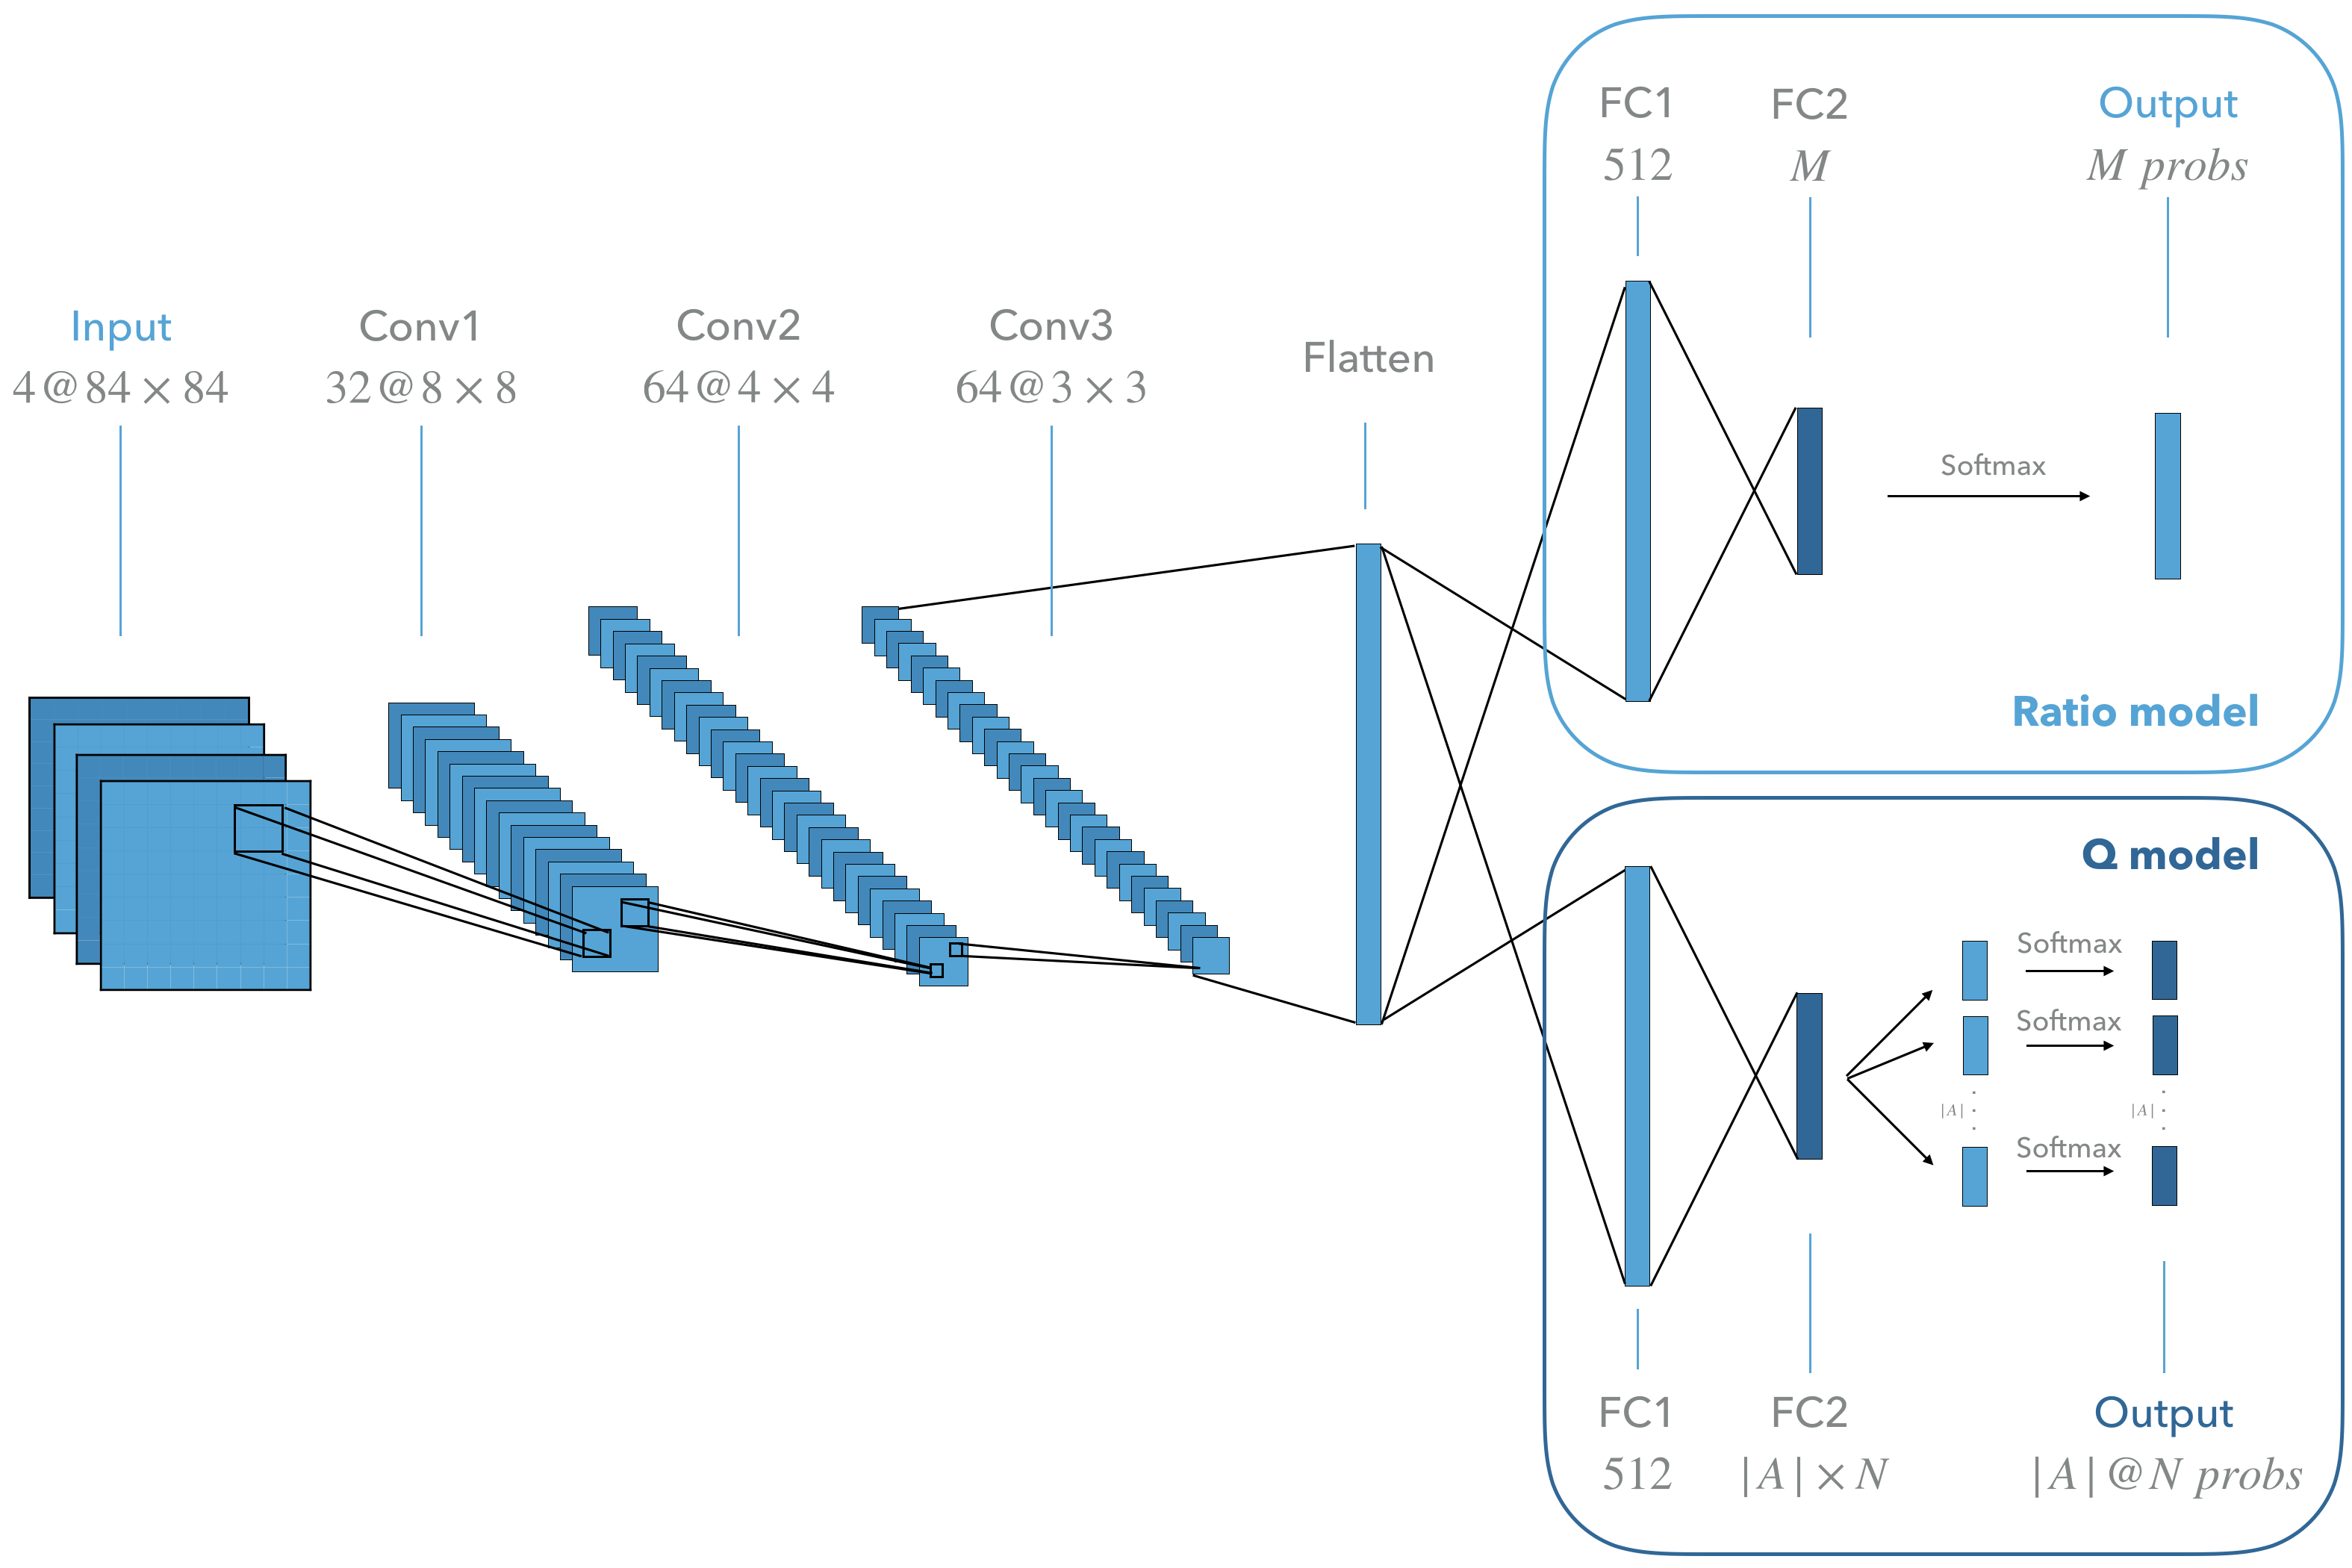
\includegraphics[width=\textwidth]{Model_Network}
    \caption{Visual representation of the Neural Network implemented in \texttt{CovariateShiftAgent} working in the ALE environment.}
    \label{fig:network}
\end{figure}

We can see in Figure \ref{fig:network} the model network architecture in detail when working with the ALE environment\cite{ALE}. Game frames are selected, grouped and preprocessed in the standard way, generating inputs which consist of a $84\times84\times4$ image. The following convolutional layers are exactly as the ones already defined in the DQN implementation\cite{DQN}:
\begin{itemize}
	\item The first hidden layer convolves 32 filters of $8\times8$ with stride 4 with the input image and applies a rectifier non-linearity -in particular, a ReLu\cite{ReLu}.
	\item The second hidden layer convolves 64 filters of $4\times4$ with stride 2, again followed by a ReLu activation function.
	\item The third and last convolutional layer convolves 64 filters of $3\times3$ with stride 1 and applies a ReLu rectifier as well, and the result is flattened.
\end{itemize}
At that point, our network is forked in two separate heads, each connected to the previous flattened layer:
\begin{itemize}
	\item On the one hand, we have the part responsible of predicting the Q value distributions, which we call the Q model. Just as the original distributional RL models\cite{DRL}, the final hidden layer is fully-connected and consists of 512 rectifier units, followed by a fully-connected linear layer with $| \A | \times N$ outputs, being $|A|$ the number of actions of the played game\footnote{The number of valid actions varied between 4 and 18 along the games of ALE environment.} and $N$ the number of fixed supports considered for the categorical Q distributions. This is re-arranged in $|A|$ groups of $N$ outputs, and applying to each of these groups of logits a Softmax layer we finally obtain the $N$ probabilities for each state-action pair.
	\item On the other hand, we have added the previously mentioned ratio model, which provides us with estimates of the covariate shift (log-)ratio distributions. As in the Q model, the final hidden layer is fully-connected and consists of 512 rectifier units. This is followed by a fully-connected linear layer that produces as mani outputs as the number of atoms $M$ of the ratio parametric model. A final softmax layer transforms the resulting logits into probabilities. 
\end{itemize}


Finally, we notice that we work with double networks\cite{DoubleNetworks} -i.e. the processes of selection and evaluation of the bootstrap action are decoupled, with online and target weights respectively; this is a usual method in Deep Reinforcement Learning that addresses a natural overestimation bias of Q-learning\cite{Double}. In our implementation, the update period for the target network is controlled by \texttt{target\_update\_period} parameter, whose value is set to $8000$ iterations just like the \texttt{RainbowAgent}\cite{Rainbow}.




\subsection{Replay Memory}

The implemented replay memory in Dopamine\cite{dopamine} is responsible of storing past transitions of the agent, acting as a windowed buffer from which training samples are drawn continuously. Consequently, there is always some degree of off-polyceness during the learning process given that the learned policy is being constantly updated.

In order to evaluate our model, however, we are interested in achieving a degree of off-polyceness as high as possible; thus, we consider the very hard setting proposed for testing the Discounted COP-TD algorithm\cite{DCOPTD}, in which:
\begin{itemize}
	\item We have a fixed behaviour policy $\mu$, the uniformly random policy;
	\item At each step, the target policy $\pi$ is the $\epsilon$-greedy policy with respect to the predicted $Q$ estimates.
\end{itemize}
On ALE\cite{ALE}, this particular setup guarantees that the generated data is significantly different from any learned policy, as we want to.

Taking the work of \cite{DCOPTD} as reference, to reweight sample transitions we have implemented a prioritized replay memory\cite{Prioritized} where priorities are simply covariate shift estimates. Nonetheless, this increases the risk of overfitting, since it reduces the effective size of the data set -those samples unlikely under policy $\pi$, which might be the vast majority due to the randomness of $\mu$, end up mostly ignored; to compensate this effect, the \texttt{replay\_capacity} is increased to $10$M frames.

Authors of \cite{DCOPTD} also explain that stability issues arise when we learn the ratio with prioritized sampling. To overcome this, at each training step two independent transition batches are sampled from the replay buffer: prioritized for the value distribution, and uniform for the covariate shift ones. In both cases, the \texttt{batch\_size} is set to 32 in our experiments.

Last, but not least, we note that initial states cannot be updated through transition samples as the training of the ratio distributions is done 'backwards'. In these cases, given that the distribution of any initial state is policy-independent, their ratio is 1; in our implementation, we take this into account by replacing the bootstrapping target with a Dirac delta centered at 1.



\subsection{Distributional Setting}

We recall Section \ref{aproxFramework}, where we described the approximation framework defined in \cite{analysisC51} to implement reproducible and scalable distributional-based RL algorithms. Let's see how we have dealt in practice with each of the key points of that framework:

\subsubsection*{Distribution Parametrisation}
Just as we considered along the theoretical framework, we select the parametric family of categorical distributions over some fixed set of supports $z_1 < \cdots < z_K$:
\begin{equation*}
	\mathcal{P} = \left\{ \sum_{i=1}^{K} p_i \delta_{z_i} \Big| p_1, \dots , p_K \geq 0, \sum_{k=1}^{K} p_k = 1 \right\}
\end{equation*}
The only difference is that our implementation allows to define supports which are not necessarily equally-spaced; in fact, apart from linear divisions of the support, in our experiments we have also taken into account exponential bins.


\subsubsection*{Stochastic Learning}
Despite the convergence results have been obtained without stochasticity, in practice it is difficult to find an example where it can be rejected. Hence, supported with the work done in \cite{analysisC51, DRLlinear} regarding stochastic updates, our implementation learns to predict covariate shift ratio estimates through transition samples of the MDP.

In particular, the practical samples for the ratio model are simply of the form $(s_t,a_t,s_{t+1})$; neither the immediate reward $r_t$ nor the next action $a_{t+1}$ are required. However, in order to define the learning rule, the ratio of policies $\rho(S^{\mu}_{s_{t+1}},A^{\mu}_{s_{t},s_{t+1}})$ must be computed; in our stochastic setting, given a transition $(s_t,a_t,s_{t+1})$, it is estimated as $\rho_t := \rho(s_t,a_t)$. Since
\begin{itemize}
    \item the \textit{behavioural policy} $\mu$ is simply the uniformly random policy, i.e. 
    \begin{equation*} \label{behaviourPolicy}
        \mu(a_t|s_t) = \frac{1}{|\mathcal{A}|} \quad \forall a \in \mathcal{A};
    \end{equation*}
    \item the \textit{target policy} $\pi$ is the $\epsilon$-greedy policy with respect to the estimated state-action q-values of the model, i.e.
    \begin{equation*} \label{targetPolicy}
        \pi_\theta (a_t|s_t) = 
        \left\{ 
            \begin{array}{lcc}
                (1-\epsilon)+\epsilon \frac{1}{|\mathcal{A}|} &   \text{if} & a_t = \text{arg max}_{a} Q_\theta(s_t,a) \\
                \epsilon \frac{1}{|\mathcal{A}|} &  \text{otherwise} &
            \end{array}
        \right. 
    \end{equation*}
\end{itemize}
we can easily obtain a computable expression:
\begin{equation} \label{policyQuotient}
        \rho_t = \frac{\pi_\theta (a_t|s_t)}{\mu(a_t|s_t)} = 
        \left\{ 
            \begin{array}{lcc}
                |\mathcal{A}|(1-\epsilon)+\epsilon  &   \text{if} & a_t = \text{arg max}_a Q_\theta(s_t,a) \\
                \epsilon  &  \text{otherwise} &
            \end{array}
        \right. 
\end{equation}

Once we have the ratio computed for each sample, it is straightforward to define both the \textit{stochastic Distributional DCOP operator} $\hat{Y}^D_{\hat{\gamma}}$ and the \textit{stochastic Log-Distributional DCOP operator} $\hat{G}_{\hat{\gamma}}$, which modify the supports of ratio distributions and log ratio distributions, respectively, according to the 1-step information contained in each sample.



\subsubsection*{Projection of Bellman Target Distribution}
In order to recover a ratio distribution within $\mathcal{P}$ after applying the stochastic operator -either $\hat{Y}^D_{\hat{\gamma}}$ or $\hat{G}_{\hat{\gamma}}$, depending on the case-, we also use the heuristic projection operator $\Pi_C$ defined in \ref{heuristicProjectionOp}; in particular, we coded it extended to finite mixtures of Dirac measures: 
	$$ \Pi_C \left( \sum_{i=1}^{N} p_i \delta_{y_i} \right) = \sum_{i=1}^{N} p_i \Pi_C ( \delta_{y_i} )	$$


We note, however, that our implementation of the function \texttt{project\_distribution($\dots$)}\footnote{This function can be found in \href{https://github.com/gbg141/dopamine/blob/master/dopamine/agents/covariate_shift/covariate_shift_agent.py}{\texttt{dopamine/agents/covariate\_shift/covariate\_shift\_agent.py}}}, responsible of performing this projection $\Pi_C$, differs from the already implemented in Dopamine; we have slightly modified it so as to allow non-equally spaced supports, thus enabling the option of running experiments with exponential bins as well.


\subsubsection*{Gradient Updates}
-A decision had to be taken about how to compute the next iterate of our stochastic approximation. Attending to what we have shown in our theoretical framework, defining a gradient update based on a Cramér loss seem to be the most appropriate solution given that we have implemented the Cramér projection $\Pi_C$. However, we finally decided to imitate the original C51 agent and perform a single step of gradient descent on the Kullback-Leibler divergence of the predicted distribution from the target one with respect to the parameters of the prediction.

The reasons behind our decision are purely practical; despite there is no convergence guarantee of C51 due to this KL divergence step, so far its experimental results\cite{DRL} are much better than those that strictly rely on the theoretical framework\cite{DRLlinear}. Hence, as we now seek for the best performance possible of our Distributional Covariate Shift approach, we kind of ignore that part of the theory and implement the KL gradient update for generating the new estimates of our \texttt{CovariateShiftAgent}.
 




\subsection{Categorical Distributional DCOP-TD}

With all the main ingredients of our implementation already detailed in previous sections, we simply want to summarize the steps that conform our distributional DCOP-TD algorithms. To begin with, we show in Algorithm \ref{alg:CatDistDCOP-TD} the Categorical Distributional $\hat{\gamma}$-Discounted COP-TD main process, where 
\begin{itemize}
	\item $\{x_K\}$ is the set of atoms that define our categorical parametric family $\mathcal{P}$
	\item we denote by $\theta$ and $\bar{\theta}$ the weights of the online and target networks, respectively;
	\item $\{p_{{\theta}_{t},K}(s)\}$ and $\{p_{\bar{\theta}_{t},K}(s)\}$ are, respectively, the set of probability outputs of the online and target networks for a state $s\in \Sspace$ at a training time step $t$.
	\item $\hat{\epsilon} \in [0,1]$ comes from the definition of the $\epsilon$-greedy policy $\pi_{\bar{\theta}}$; in practice, however, it can be controlled apart by  an extra hyper-parameter (\texttt{quotient\_epsilon}).
	\item $(f_{a,b})_\#$ represents the application to each element of the support of an affine shift map $f_{a,b} : \R \rightarrow \R$ defined by $f_{a,b}(y) := a + b y$; in particular, note that $Y_{\hat{\gamma}}^D X(s) := (f_{\cdot,\hat{\gamma}\rho})_{\#} X(s)$
\end{itemize}


\vspace{\fill}

\setlength{\algomargin}{1.5em}
\SetAlCapHSkip{0em}
\begin{algorithm}[h!]
\caption{Categorical Distributional DCOP-TD} \label{alg:CatDistDCOP-TD}
\DontPrintSemicolon
\SetKwComment{CustomComment}{\#}{}
\SetKwInput{KwIn}{\hspace{-1.5em} Input}
\SetKwInput{KwOut}{\hspace{-1.5em} Output}
\SetKwInOut{Require}{\hspace{-1.5em} Require}
\Require{Estimates $X_{{\theta}_{t}}(s) = \sum_{k=1}^K p_{{\theta}_{t},k}(s) \delta_{x_k}$ and $X_{\bar{\theta}_{t}}(s) = \sum_{k=1}^K p_{\bar{\theta}_{t},k}(s) \delta_{x_k}$ for each $s\in\Sspace$}
\KwIn{A sample transition $(s_{i},a_{i}, s_{i+1})$}
	\CustomComment{Compute policy ratio}
    \uIf{$a_t =  \textnormal{arg max}_a Q_{\bar{\theta}}(s_{i},a)$ }{
    	$\rho_i \leftarrow |\mathcal{A}|(1-\hat{\epsilon})+\hat{\epsilon} $ \;}
    \Else{
    	$\rho_i \leftarrow \hat{\epsilon} / |\mathcal{A}| $ \;}
    \CustomComment{Compute distributional ratio target}
    $\widehat{X}_{*}(s_{i+1}) \leftarrow Y_{\hat{\gamma}}^D X_{\bar{\theta}_{t}}(s_i)$\;
    \CustomComment{Project target onto support}
    $\widehat{X}_{t}(s_{i+1}) \leftarrow \Pi_C \widehat{X}_{*}(s_{i+1})$\;
    \CustomComment{Compute KL loss}
    \textnormal{Find gradient }$ \textnormal{KL} \left( \widehat{X}_{t}(s_{i+1}) || X_{{\theta}_{t}}(s_{i+1}) \right) $\; 
    \textnormal{Update online weights }${\theta}_{t+1} $\; 
    \CustomComment{Update target network if required}
    $\bar{\theta}_{t+1} \leftarrow {\theta}_{t+1}$ \textbf{ if } $t \ \% \ $\texttt{target\_update\_period}$\ =0$ \textbf{ else } $\bar{\theta}_{t}$\;
\KwOut{New estimates $X_{{\theta}_{t+1}}(s) = \sum_{k=1}^K p_{{\theta}_{t+1},k}(s) \delta_{x_k}$ and $X_{\bar{\theta}_{t+1}}(s) = \sum_{k=1}^K p_{\bar{\theta}_{t+1},k}(s) \delta_{x_k}$ for each $s \in \Sspace$ \linebreak 
	Ratio estimates $c_{\bar{\theta}_{t+1}}(s) = \sum_{k=1}^K p_{\bar{\theta}_{t+1},k} (s) x_k$  }

\end{algorithm}

\clearpage

\subsection{Categorical Log-Distributional DCOP-TD}

Finally, we present in Algorithm \ref{alg:CatLogDistDCOP-TD} the sketch of our Categorical Log-Distributional DCOP-TD algorithm. The observations made in previous Section apply here, where now $\{w_K\}$ is the support and $G_{\hat{\gamma}} W(s) =$ $(f_{\log(\rho),\hat{\gamma}})_{\#} W(s)$. In fact, as one can easily see, the steps are equivalent to those of the multiplicative case.



\setlength{\algomargin}{1.5em}
\SetAlCapHSkip{0em}
\begin{algorithm}[h!]
\caption{Categorical Log-Distributional DCOP-TD} \label{alg:CatLogDistDCOP-TD}
\DontPrintSemicolon
\SetKwComment{CustomComment}{\#}{}
\SetKwInput{KwIn}{\hspace{-1.5em} Input}
\SetKwInput{KwOut}{\hspace{-1.5em} Output}
\SetKwInOut{Require}{\hspace{-1.5em} Require}
\Require{Estimates $W_{{\theta}_{t}}(s) = \sum_{k=1}^K p_{{\theta}_{t},k}(s) \delta_{w_k}$ and $W_{\bar{\theta}_{t}}(s) = \sum_{k=1}^K p_{\bar{\theta}_{t},k}(s) \delta_{w_k}$ for each $s\in\Sspace$}
\KwIn{A sample transition $(s_{i},a_{i}, s_{i+1})$}
	\CustomComment{Compute the log policy ratio}
    \uIf{$a_t =  \textnormal{arg max}_a Q_{\bar{\theta}}(s_{i},a)$ }{
    	$\log (\rho_i) \leftarrow \log \left( |\mathcal{A}|(1-\hat{\epsilon})+\hat{\epsilon} \right) $ \;}
    \Else{
    	$\log (\rho_i) \leftarrow \left(\hat{\epsilon} / |\mathcal{A}| \right)$ \;}
    \CustomComment{Compute distributional log-ratio target}
    $\widehat{W}_{*}(s_{i+1}) \leftarrow (f_{\log (\rho_i),\hat{\gamma}})_{\#} W_{\bar{\theta}_{t}}(s_i)$\;
    \CustomComment{Project target onto support}
    $\widehat{W}_{t}(s_{i+1}) \leftarrow \Pi_C \widehat{W}_{*}(s_{i+1})$\;
    \CustomComment{Compute KL loss}
    \textnormal{Find gradient }$ \textnormal{KL} \left( \widehat{W}_{t}(s_{i+1}) || W_{{\theta}_{t}}(s_{i+1}) \right) $\; 
    \textnormal{Update online weights }${\theta}_{t+1} $\; 
    \CustomComment{Update target network if required}
    $\bar{\theta}_{t+1} \leftarrow {\theta}_{t+1}$ \textbf{ if } $t \ \% \ $\texttt{target\_update\_period}$\ =0$ \textbf{ else } $\bar{\theta}_{t}$\;
\KwOut{New estimates $W_{{\theta}_{t+1}}(s) = \sum_{k=1}^K p_{{\theta}_{t+1},k}(s) \delta_{w_k}$ and $W_{\bar{\theta}_{t+1}}(s) = \sum_{k=1}^K p_{\bar{\theta}_{t+1},k}(s) \delta_{w_k}$ for each $s \in \Sspace$  \linebreak 
	Ratio estimates $c_{\bar{\theta}_{t+1}}(s) = \sum_{k=1}^K p_{\bar{\theta}_{t+1},k} (s) \exp (w_k)$ }
\end{algorithm}

We note that we can easily get covariate shift estimates -which we recall are used as priorities for training the $Q$ model- by exponentiating log-ratio distributions and taking its mean; in practice, as the support is fixed, we simply compute the exponentiated support at the beginning, and compute its weighted mean by the corresponding probabilities of log-ratio distributions.


\newpage 
\thispagestyle{plain}
\section{Evaluation of the Proposal}

\begin{itemize}
	\item Importance of Ratio Intervals
	\item Computational cost: limited fine-tuning, 100 iterations max
	\item Weight loss
	\item Summary of section
\end{itemize}




\subsection*{Linear vs Exponential Bins in Multiplicative case}

Abliation Seaquest:

\begin{figure}[h]
    \centering
    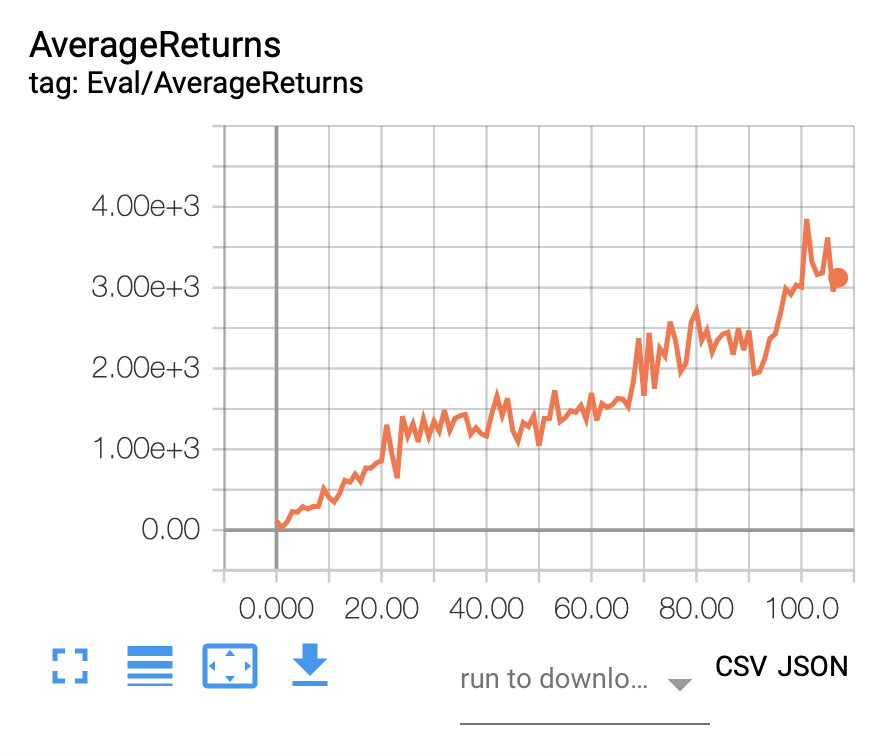
\includegraphics[width=0.5\textwidth]{multiplicativeExpBins}
    \caption{multiplicativeExpBins}
    \label{fig:multiplicativeExpBins}
\end{figure}

\begin{figure}[h]
    \centering
    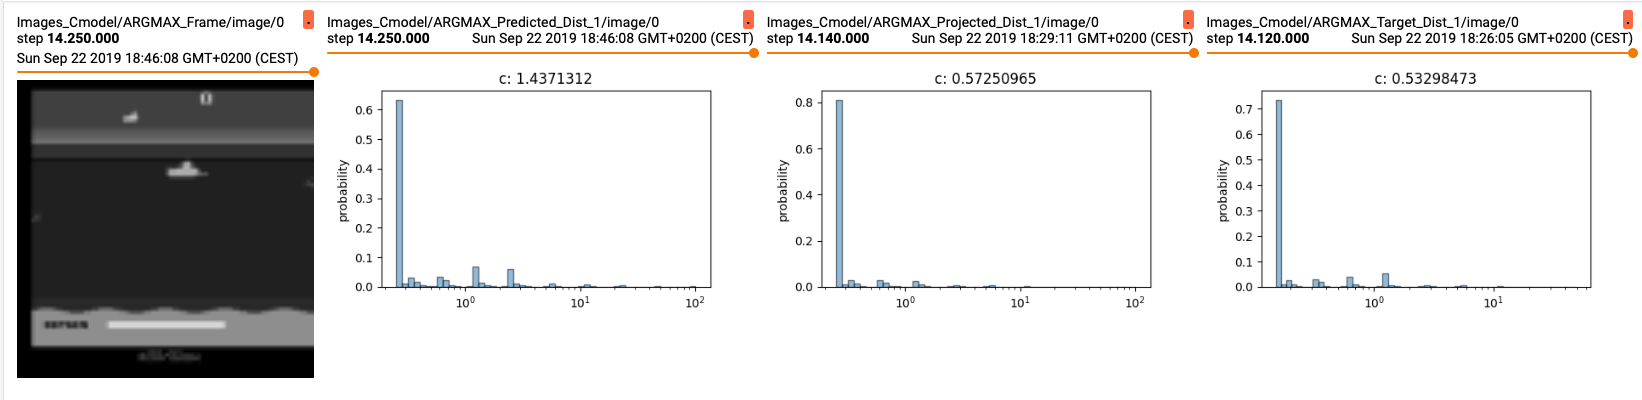
\includegraphics[width=\textwidth]{multiplicativeExpBinsProcess}
    \caption{multiplicativeExpBinsProcess}
    \label{fig:multiplicativeExpBinsProcess}
\end{figure}

\begin{figure}[h]
    \centering
    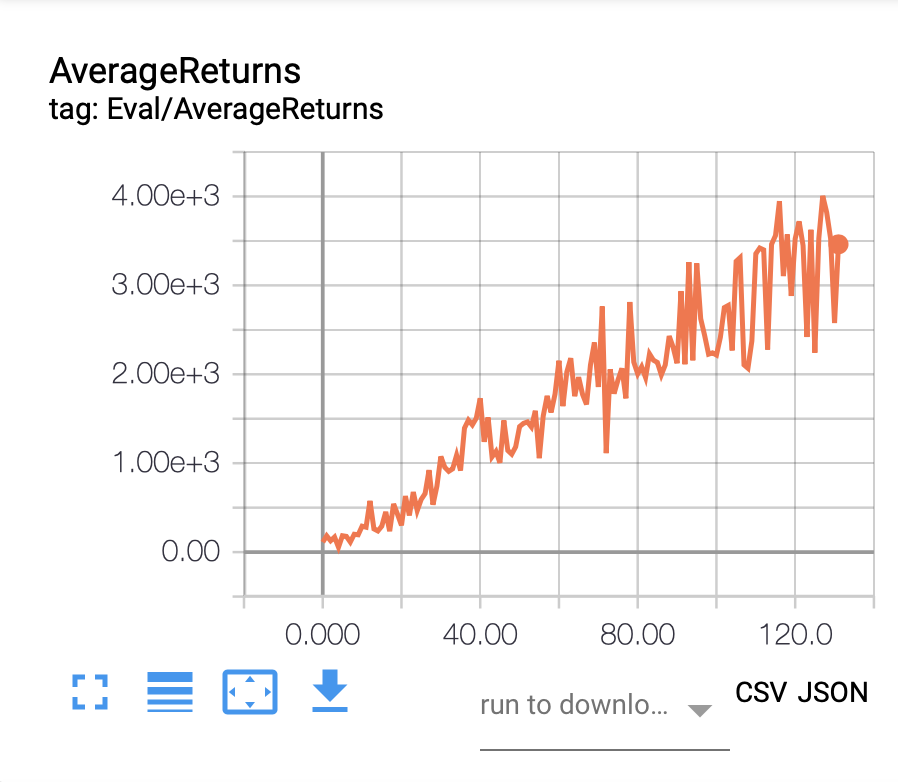
\includegraphics[width=0.5\textwidth]{multiplicativeLinBins}
    \caption{multiplicativeLinBins}
    \label{fig:multiplicativeLinBins}
\end{figure}

\begin{figure}[h]
    \centering
    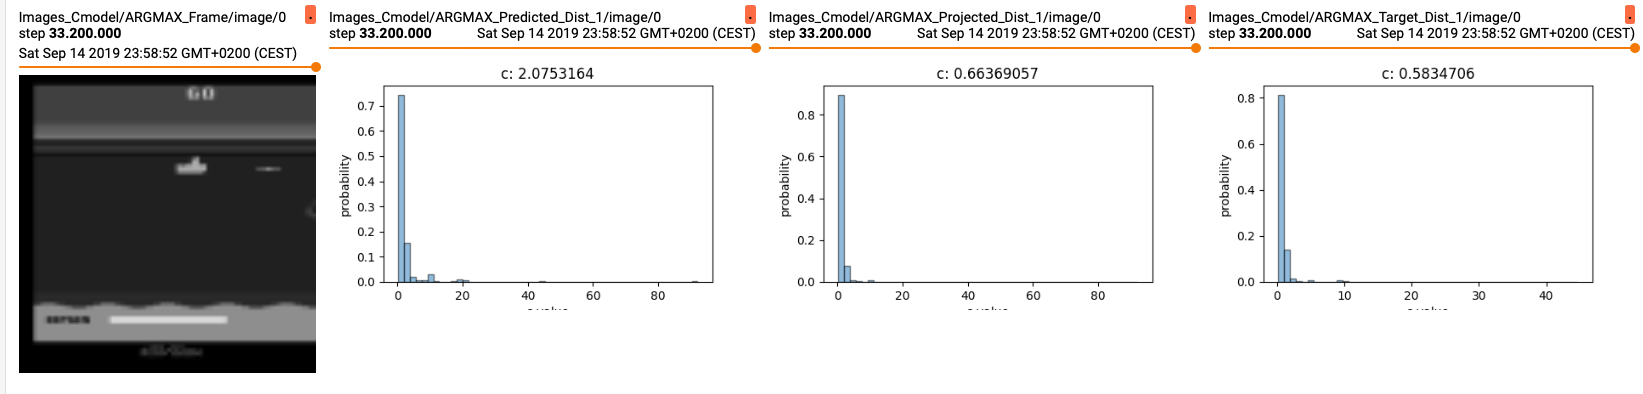
\includegraphics[width=\textwidth]{multiplicativeLinBinsProcess}
    \caption{multiplicativeLinBinsProcess}
    \label{fig:multiplicativeLinBinsProcess}
\end{figure}

\clearpage

\subsection*{Log-Distributional Approach}


\subsection*{Qualitative Evaluation of the Learned Ratios}

\begin{figure}[h]
    \centering
    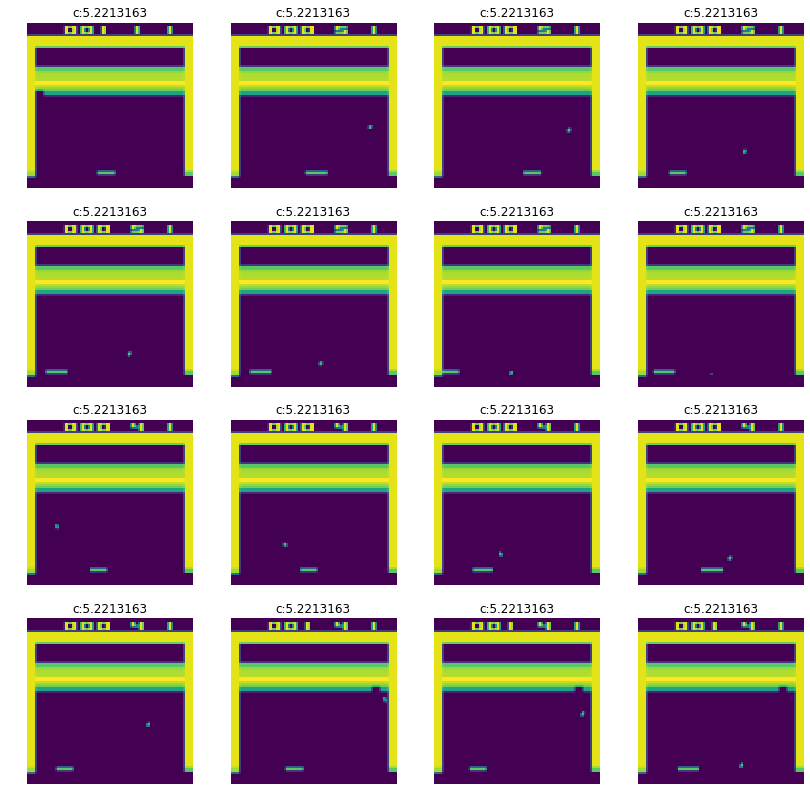
\includegraphics[width=\textwidth]{MaxBreakout}
    \caption{MaxBreakout}
    \label{fig:MaxBreakout}
\end{figure}

\begin{figure}[h]
    \centering
    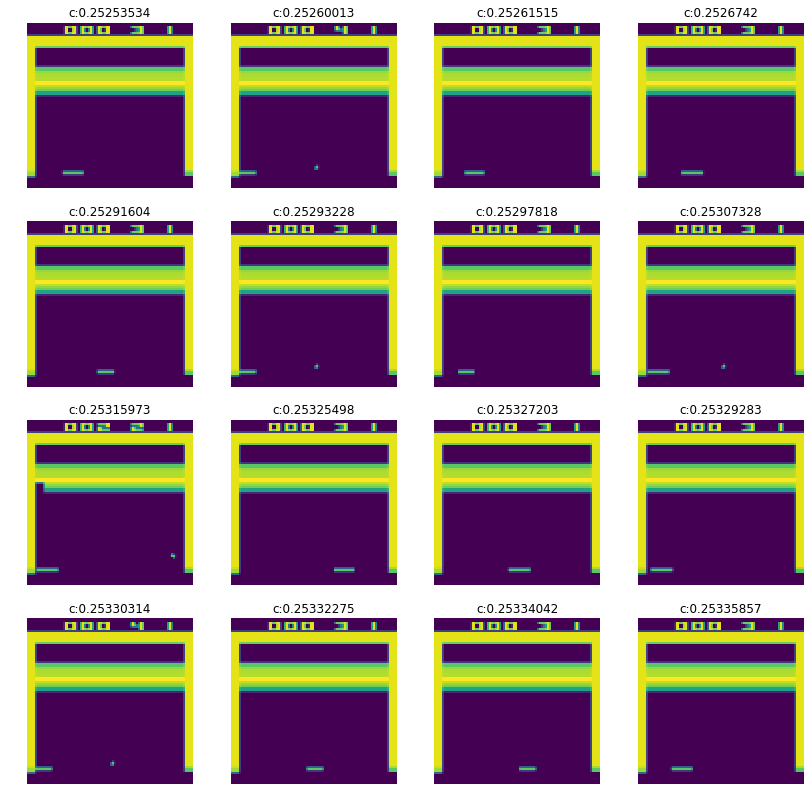
\includegraphics[width=\textwidth]{MinBreakout}
    \caption{MinBreakout}
    \label{fig:MinBreakout}
\end{figure}

\clearpage

\newpage

\thispagestyle{plain}
\section{Conclusions}


\newpage

\appendix
\pagestyle{fancy}
\renewcommand{\sectionmark}[1]{\markboth{#1}{}}
\renewcommand{\subsectionmark}[1]{\markright{\thesubsection.\quad #1}}

\thispagestyle{plain}
\section*{Appendix}
\addcontentsline{toc}{section}{Appendix}
\sectionmark{Appendix}

\setcounter{section}{1}
\setcounter{theorem}{0}
\setcounter{definition}{0}
\setcounter{equation}{0}

\subsection{Mixture Distributions}

\begin{remark}
All random variables presented in this document are considered to be real-valued, i.e. their measurable space is $E= \R$. 
\end{remark}

A random variable $Y$ is a mixture distribution if it is derived from a collection of other random variables $\{X_i\}$, $i\in \{1, \dots, N\}$, (named mixture components) in such a way that the combination of these parent distributions is driven according to a certain distribution $A$ (called mixing distribution). $A$ encapsulates the mixture weights $\alpha_i \sim A$, $i\in \{1, \dots, N\}$, which represent the probabilities of each individual mixture component $X_i$. 

The mixture distribution $Y$ can be defined in terms of its density function $f_Y$, which is the resulting $\alpha$-convex combination of the mixture components' density functions:
\begin{equation} \label{mixtureDef}
    f_{Y} (x) = \sum_{i=1}^{N} \alpha _i f_{X_i}(x)
\end{equation}

Let's present some interesting properties of mixture distributions:

\begin{mixtureProperty} \label{mixtureProperty1}
	The expectation of the mixture distribution $Y$ is the convex combination of expectations of each mixture component: 
    \begin{equation} \label{mixtureProperty1eq}
    \begin{split}
        \E [Y] &= \int_{-\infty}^{\infty} x f_{Y}(x) dx = \int_{-\infty}^{\infty} x \sum_{i=1}^{N} \alpha_i f_{X_i}(x) dx \\
        &= \sum_{i=1}^{N} \alpha_i \int_{-\infty}^{\infty} x f_{X_i}(x) dx \\
        &= \sum_{i=1}^{N} \alpha_i \E [X_i]
    \end{split}
    \end{equation}
\end{mixtureProperty}


\begin{mixtureProperty} \label{mixtureProperty2}
	Let be $Z$ a mixture distribution with mixture components $\{g_i(X_i)\}$, $i\in \{1, \dots, N\}$ and mixing weights $\alpha_i \sim A$
    \begin{equation} \label{mixtureProperty2eq}
        \E [Z] = \sum_{i=1}^{N} \alpha_i \E [g_i(X_i)]
    \end{equation}
\end{mixtureProperty}


\begin{mixtureProperty} \label{mixtureProperty3}
	Let be $Z=g(Y)$, being $Y$ a mixture distribution with mixture components $\{X_i\}$, $i\in \{1, \dots, N\}$, and $g$ a monotonic, invertible and differentiable function. Then we have that $Z$ is a mixture distribution whose expectation is
    \begin{equation} \label{mixtureProperty3eq}
        \begin{split}
        \E [Z] &= \int_{-\infty}^{\infty} g(x) f_{Y}(x) dx \\
        &= \int_{-\infty}^{\infty} g(x) \left( \sum_{i=1}^{N} \alpha_i f_{X_i}(x)\right) dx = \sum_{i=1}^{N} \alpha_i \int_{-\infty}^{\infty} g(x) f_{X_i}(x) dx \\
        &= \sum_{i=1}^{N} \alpha_i \E [g(X_i)]
        \end{split}
    \end{equation}
    Note that in both the first and last steps the so-called Law of the Unconscious Statistician has been applied, which states that
    \begin{equation} \label{LOTUS}
    	\E [g(X)] = \int_{-\infty}^{\infty} y f_{g(X)}(y) dy  = \int_{-\infty}^{\infty} g(x) f_{X}(x) dx
    \end{equation}

\end{mixtureProperty}

We emphasize the relevance of \textbf{Property \ref{mixtureProperty3}}. In distributional TD learning, the distribution mixture plays the role of the expectation in expected TD. But while $\E[g(x)] \not= g(\E[x])$, we can interchange mixtures and functions. This allows us to circumvent Jensen's inequalities.

\begin{comment}
\subsubsection*{Sum of Distributions} 
	
The sum of two independent random variables $X_1$ and $X_2$, $Y=X_1 + X_2$, results in a random variable whose density function is the convolution of the density functions of each summand
\begin{equation}
	f_{Y}(y) = \int_{-\infty}^{\infty} f_{X_1}(y-x) f_{X_2}(x)dx = \left(f_{X_1}* f_{X_2} \right) (y)
\end{equation}

In the general case, considering a collection $\{X_i\}$, $i\in \{1, \dots, N\}$, of independent random variables, the density function of the random variable $Y = \sum_{i=1}^{N} X_i $
can be expressed as the convolution of all the individual density functions:
\begin{equation}
	f_{Y} (x) = \left(f_{X_1} * \cdots * f_{X_N} \right) (x)
\end{equation}

Convolutions are linear operators.
\end{comment}





\subsection{Metrics over Distributions} \label{metrics}


\subsubsection{Kullback-Leibler Divergence}

\begin{definition}
	Let be $\nu_1, \nu_2 \in \mathscr{P}(\R)$ two probability distributions. The Kullback-Leibler (KL) divergence of $\nu_1$ from $\nu_2$ is defined as
	\begin{equation*}
		D_{KL} (\nu_1,\nu_2) = \int_{-\infty}^{\infty} \nu_1(x) \log \frac{\nu_1(x)}{\nu_2(x)} dx
	\end{equation*}
\end{definition}

\subsubsection{Wasserstein}

\begin{definition}
	The Wasserstein distance $d_p$, for $p\in [1,\infty)$, between two distributions $\nu_1, \nu_2 \in \mathscr{P}(\R)$, with cumulative distribution functions $F_{\nu_1}, F_{\nu_2}$ respectively, can be defined by:
	\begin{equation*}
		d_p(\nu_1,\nu_2) = \left( \int_{\R} | F_{\nu_1}^{-1}(u) - F_{\nu_2}^{-1}(u)|^p du \right) ^{1/p}
	\end{equation*}
	Further, the supremum-Wasserstein metric $\bar{d}_p$ is defined between two value distribution functions $Z, Z' \in \Z$ by
	\begin{equation*}
		\bar{d}_p(Z,Z') = \sup_{(s,a) \in \Sspace \times \A} d_p(Z(s,a), Z'(s,a))
	\end{equation*}
\end{definition}


\subsubsection{Cramér}

\begin{definition}
	The Cramér distance $\ell_2$ between two distributions $\nu_1, \nu_2 \in \mathscr{P}(\R)$, with cumulative distribution functions $F_{\nu_1}, F_{\nu_2}$ respectively, is defined by:
	\begin{equation*}
		\ell_2(\nu_1,\nu_2) = \left( \int_{\R} (F_{\nu_1}(x) - F_{\nu_2}(x))^2dx \right) ^{1/2}
	\end{equation*}
	Further, the supremum-Cramér metric $\bar{\ell}_2$ is defined between two value distribution functions $Z, Z' \in \Z$ by
	\begin{equation*}
		\bar{\ell}_2(Z,Z') = \sup_{(s,a) \in \Sspace \times \A} \ell_2(Z(s,a), Z'(s,a))
	\end{equation*}
\end{definition}


%\subsubsection{Generalized Cramér}





\subsection{Contraction Mappings} \label{contractionTheory}



\subsection{Implementation Details}

TODO!!!

Our baseline is the C51 distributional reinforcement learning agent\cite{DRL} within Dopamine framework\cite{dopamine}. We use published hyperparameters unless otherwise noted. We augment the C51 network by adding an extra head, the distributional ratio model $X(s)$, to the final convolutional layer, whose role is to predict the distribution of the ratio $d_\pi / d_\mu$ . This model consists of a two-layer fully-connected network, with as many outputs as the number of atoms $M$ of the parametric model. A final softmax layer transforms the resulting logits into probabilities. 

\newpage

\thispagestyle{plain}
\addcontentsline{toc}{section}{Referencias}\sectionmark{Referencias}
\begin{thebibliography}{50}

	\bibitem{DRL} M. G. Bellamare, W. Dabney and R. Munos. A Distributional Perspective on Reinforcement Learning.
	\bibitem{COPTD} A. Hallak and S. Mannor. Consistent On-Line Off-Policy Evaluation.
	\bibitem{DCOPTD} C. Gelada and M. G. Bellamare. Off-Policy Deep Reinforcement Learning by Bootstrapping the Covariate Shift.
	\bibitem{unichain}  S. P. Meyn and R. L. Tweedie. Markov chains and stochastic stability. 2012.
	\bibitem{TD} Sutton, R. S., and Barto, A. G. 2018. Reinforcement learning: An introduction. MIT Press, 2nd edition.
	\bibitem{projectedBellman} Tsitsiklis, J. N., and Van Roy, B. 1997. An analysis of temporal-difference learning with function approximation. IEEE Transactions on Automatic Control 42(5):674–690.
	\bibitem{dopamine} Dopamine: {A} Research Framework for Deep Reinforcement Learning. \url{https://github.com/google/dopamine}
	\bibitem{rlformulation} Bertsekas, D. and Tsitsiklis, J. Neuro-Dynamic Programming. Athena Scientific, 1996.
	\bibitem{ETD} Sutton, R. S., Mahmood, A. R., and White, M. An emphatic approach to the problem of off-policy temporal- difference learning. arXiv:1503.04269, 2015.
	\bibitem{generalizedETD} Hallak, Assaf, Tamar, Aviv, Munos, Remi, and Mannor, Shie. Generalized emphatic temporal difference learning: Bias-variance analysis. arXiv preprint arXiv:1509.05172, 2015.
	\bibitem{DRLlinear} Marc G. Bellemare, Nicolas Le Roux, Pablo Samuel Castro and Subhodeep Moitra. Distributional reinforcement learning with linear function approximation
	\bibitem{analysisC51} Rowland, Mark, Bellemare, Marc G, Dabney, Will, Munos, Rémi, and Teh, Yee Whye. An analysis of categorical distributional reinforcement learning. In Proceedings of the International Conference on Artificial Intelligence and Statistics, 2018.
	\bibitem{firstDistributional} Jaquette, Stratton C. Markov decision processes with a new opti- mality criterion: Discrete time. The Annals of Statistics, 1(3): 496–505, 1973.
	\bibitem{ALE} Bellemare, Marc G, Naddaf, Yavar, Veness, Joel, and Bowling, Michael. The arcade learning environment: An evaluation plat- form for general agents. Journal of Artificial Intelligence Re- search, 47:253–279, 2013.
	\bibitem{DQN} Mnih, V.; Kavukcuoglu, K.; Silver, D.; Rusu, A. A.; Veness, J.; Bellemare, M. G.; Graves, A.; Riedmiller, M.; Fidjeland, A. K.; Ostrovski, G.; Petersen, S.; Beattie, C.; Sadik, A.; Antonoglou, I.; King, H.; Kumaran, D.; Wierstra, D.; Legg, S; and Hassabis, D. 2015. Human-level control through deep reinforcement learning. Nature 518(7540):529–533.
	\bibitem{ReLu} Nair, V. and Hinton, G. E. Rectified linear units improve restricted Boltzmann machines. Proc. Int. Conf. Mach. Learn. 807–814 (2010).
	\bibitem{Rainbow} Hessel, Matteo, Modayil, Joseph, van Hasselt, Hado, Schaul, Tom, Ostrovski, Georg, Dabney, Will, Hor- gan, Dan, Piot, Bilal, Azar, Mohammad, and Silver, David. Rainbow: Combining improvements in deep reinforcement learning. In Proceedings of the AAAI Conference on Artificial Intelligence, 2018.
	\bibitem{DoubleNetworks} van Hasselt, H.; Guez, A.; and Silver, D. 2016. Deep re- inforcement learning with double Q-learning. In Proc. of AAAI, 2094–2100.
	\bibitem{Double} van Hasselt, H. 2010. Double Q-learning. In Advances in Neural Information Processing Systems 23, 2613–2621.
	\bibitem{Prioritized} Schaul, T.; Quan, J.; Antonoglou, I.; and Silver, D. 2016. Prioritized experience replay. In International Conference on Learning Representations.





\end{thebibliography}


%\thispagestyle{plain}\nocite{*}\addcontentsline{toc}{section}{Referencias}\sectionmark{Referencias}\bibliography{Bibliografia} \bibliographystyle{unsrt}

\end{document}